%%
%% Copyright 2007, 2008, 2009 Elsevier Ltd
%%
%% This file is part of the 'Elsarticle Bundle'.
%% ---------------------------------------------
%%
%% It may be distributed under the conditions of the LaTeX Project Public
%% License, either version 1.2 of this license or (at your option) any
%% later version.  The latest version of this license is in
%%    http://www.latex-project.org/lppl.txt
%% and version 1.2 or later is part of all distributions of LaTeX
%% version 1999/12/01 or later.
%%
%% The list of all files belonging to the 'Elsarticle Bundle' is
%% given in the file `manifest.txt'.
%%

%% Template article for Elsevier's document class `elsarticle'
%% with harvard style bibliographic references
%% SP 2008/03/01
%%
%%
%%
%% $Id: elsarticle-template-harv.tex 4 2009-10-24 08:22:58Z rishi $
%%
%%
%\documentclass[final,3p,authoryear,times,twocolumn]{elsarticle}
\documentclass[preprint,authoryear,12pt,dvipdfm]{elsarticle}

%% Use the option review to obtain double line spacing
%% \documentclass[authoryear,preprint,review,12pt]{elsarticle}

%% Use the options 1p,twocolumn; 3p; 3p,twocolumn; 5p; or 5p,twocolumn
%% for a journal layout:
%% \documentclass[final,authoryear,1p,times]{elsarticle}
%% \documentclass[final,authoryear,1p,times,twocolumn]{elsarticle}
%% \documentclass[final,authoryear,3p,times]{elsarticle}
%% \documentclass[final,authoryear,3p,times,twocolumn]{elsarticle}
%% \documentclass[final,authoryear,5p,times]{elsarticle}
%% \documentclass[final,authoryear,5p,times,twocolumn]{elsarticle}

%% if you use PostScript figures in your article
%% use the graphics package for simple commands
%% \usepackage{graphics}
%% or use the graphicx package for more complicated commands
%% \usepackage{graphicx}
%% or use the epsfig package if you prefer to use the old commands
%% \usepackage{epsfig}

%% The amssymb package provides various useful mathematical symbols
\usepackage{amssymb}
%% The amsthm package provides extended theorem environments
%% \usepackage{amsthm}
\usepackage[utf8]{inputenc}
\usepackage{booktabs}
\usepackage{verbatim}
\usepackage{filecontents}


\begin{filecontents}{\jobname.bib}
@article{weiser91,
    author  = "Mark Weiser",
    title   = "The Computer for the 21st Century",
    year    = "1991",
    journal = "Scientific America",
    pages   = "94--104",
}

@article{weiser96,
    author  = "Mark Weiser and John Seely Brown",
    title   = "Designing Calm Technology",
    month   = "July",
    year    = "1996",
    journal = "PowerGrid Journal",
}

@article{dey2001,
    author  = "A. Dey",
    title   = "Understanding and Using Context",
    journal = "Personal and Ubiquitous Computing", 
    volume  = "6",
    number  = "1",
    year    = "2001", 
    pages   = "4--7"
}

@article{dey2001b,
 author = {Dey, Anind K. and Abowd, Gregory D. and Salber, Daniel},
 title = {A conceptual framework and a toolkit for supporting the rapid prototyping of context-aware applications},
 journal = {Hum.-Comput. Interact.},
 issue_date = {December 2001},
 volume = {16},
 number = {2},
 month = dec,
 year = {2001},
 issn = {0737-0024},
 pages = {97--166},
 numpages = {70},
 acmid = {1463110},
 publisher = {L. Erlbaum Associates Inc.},
 address = {Hillsdale, NJ, USA},
} 


@inproceedings{abowd99,
 author = {Abowd, Gregory D. and Dey, Anind K. and Brown, Peter J. and Davies, Nigel and Smith, Mark and Steggles, Pete},
 title = {Towards a Better Understanding of Context and Context-Awareness},
 booktitle = {Proceedings of the 1st international symposium on Handheld and Ubiquitous Computing},
 series = {HUC '99},
 year = {1999},
 isbn = {3-540-66550-1},
 location = {Karlsruhe, Germany},
 pages = {304--307},
 numpages = {4},
 acmid = {743843},
 publisher = {Springer-Verlag},
 address = {London, UK},
} 

@inproceedings{schilit94,
    author = {Bill Schilit and Norman Adams and Roy Want},
    title = {Context-Aware Computing Applications},
    booktitle = {In Proceedings of the Workshop on Mobile Computing Systems and Applications},
    year = {1994},
    pages = {85--90},
    publisher = {IEEE Computer Society}
}

@article{pelep,
    author = { Darci Levis and Jorge L. V. Barbosa and Sérgio Crespo C. S. Pinto and Debora Nice Ferrari Barbosa },
    title = { Automatic Improvement of the Learner's Profile in Ubiquitous Systems },
    journal = { Braz J Inform Educ },
    volume = { 16 },
    number = { 1 },
    pages = { 29--41 },
    year = { 2008 }
}

@article{smith08,
    location = {http://www.scientificcommons.org/42583888},
    title = {Towards Truly Ubiquitous Life Annotation},
    author = {Ashley Smith and Wendy Hall and Hugh Glaser and Leslie Carr},
    year = {2008},
    abstract = {Throughout the age of information technology, we have experienced our lives getting simpler through the use of computers. Computer technology is becoming more and more integrated into our everyday routines, and as the technology becomes available we come to rely upon it. In this document we present a discussion of current technology that may be used to annotate the life of a human being, and propose a future in which diaries are obsolete in favour of computer technology and the Semantic Web. 1},
    institution = {CiteSeerX - Scientific Literature Digital Library and Search Engine [http://citeseerx.ist.psu.edu/oai2] (United States)},
}

@inproceedings{silva09,
    author = {Silva, Jader and Rosa, João and Barbosa, Jorge and Barbosa, D\'{e}bora N. F. and Palazzo, Luiz Ant\^{o}nio Moro},
    title = {Content distribution in trail-aware environments},
    booktitle = {Proceedings of the XV Brazilian Symposium on Multimedia and the Web},
    series = {WebMedia '09},
    year = {2009},
    isbn = {978-1-60558-880-3},
    location = {Fortaleza, Cear\á, Brazil},
    pages = {15:1--15:8},
    articleno = {15},
    numpages = {8},
    acmid = {1858492},
    publisher = {ACM},
    address = {New York, NY, USA},
    keywords = {context management, mobile computing, trails},
} 

@article{starner96,
    author = {Thad Starner and Bradley Rhodes and Joshua Weaver and Alex Pentland},
    title = {Human-powered wearable computing},
    journal = {IBM Systems Journal},
    year = {1996},
    volume = {35},
    pages = {618--629}
}

@inproceedings{yamim02,
    author = {Yamin, Adenauer C. and Augustin, Iara and Barbosa, Jorge L. V. and Geyer, Cl\'{a}udio F. R.},
    title = {ISAM: a pervasive view in distributed mobile computing},
    booktitle = {Proceedings of the IFIP TC6 / WG6.2 \& WG6.7 Conference on Network Control and Engineering for QoS, Security and Mobility},
    year = {2002},
    isbn = {1-4020-7268-6},
    pages = {431--436},
    numpages = {6},
    acmid = {716373},
    publisher = {Kluwer, B.V.},
    address = {Deventer, The Netherlands, The Netherlands},
} 

@misc{bbc10,
    author = {BBC},
    title = {Over 5 billion mobile phone connections worldwide},
    year = {2010},
    NOTE = "\texttt{http://www.bbc.co.uk/news/10569081}",
}

@misc{acm10,
    author = {ACM},
    title = {ACM Computing Classification System},
    year = {2012},
    note = "\texttt{http://www.acm.org/class/2012}",
}

@inproceedings{chellouche10,
    author = {Chellouche, Soraya Ait and Arnaud, Julien and N\'{e}gru, Daniel},
    title = {Flexible user profile management for context-aware ubiquitous environments},
    booktitle = {Proceedings of the 7th IEEE conference on Consumer communications and networking conference},
    series = {CCNC'10},
    year = {2010},
    isbn = {978-1-4244-5175-3},
    location = {Las Vegas, Nevada, USA},
    pages = {980--984},
    numpages = {5},
    acmid = {1834438},
    publisher = {IEEE Press},
    address = {Piscataway, NJ, USA},
    keywords = {context-awareness, middleware, personalized services, ubiquitous environments, user profile},
} 

@article{sutterer07, 
    author = {Michael Sutterer and Olivier Coutand and Olaf Droegehorn and Klaus David and Kees van der Sluijs}, 
    title = {Managing and Delivering Context-Dependent User Preferences in Ubiquitous Computing Environments},
    journal ={Applications and the Internet Workshops, IEEE/IPSJ International Symposium on},
    volume = {0},
    isbn = {0-7695-2757-4},
    year = {2007},
    pages = {4},
    publisher = {IEEE Computer Society},
    address = {Los Alamitos, CA, USA}
}

@inproceedings{korth07,
    author = {Alexander Korth and Till Plumbaum},
    booktitle = {Information Reuse and Integration, 2007. IRI 2007. IEEE International Conference on Information Reuse and Integration},
    interhash = {56d8968d18a459ea7a1ad484c8dda2d6},
    intrahash = {7e7626829a79c7d70fefd8d5824e6fb8},
    pages = {291-297},
    title = {A Framework for Ubiquitous User Modeling},
    year = 2007,
    keywords = {jabref:noKeywordAssigned},
    added-at = {2009-03-16T11:46:26.000+0100},
    month = {August}
}


@inproceedings{silva08,
    author = {da Silva, Douglas Michaelsen and Barbosa, Jorge and Vieira, Renata},
    title = {OCtoPUS: um modelo para classificação de perfil de usuários usando trilhas em sistemas ubíquos},
    booktitle = {Companion Proceedings of the XIV Brazilian Symposium on Multimedia and the Web},
    series = {WebMedia '08},
    year = {2008},
    isbn = {978-85-7669-199-0},
    location = {Vila Velha, Esp\írito Santo, Brazil},
    pages = {185--188},
    numpages = {4},
    acmid = {1810036},
    publisher = {ACM},
    address = {New York, NY, USA},
    keywords = {intelligent agents, semantic web, trail, ubiquitous computing},
} 

@InProceedings{viviani10,
  title         = {{A Survey on User Modeling in Multi-Application 
    Environments}},
  author        = {Marco Viviani and Nadia Bennani and Elod 
    Egyed-Zsigmond},
  year          = {2010},
  month         = aug,
  booktitle     = {The Third International Conference on Advances in 
    Human-oriented and Personalized Mechanisms, Technologies, and Services 
    CENTRIC'10},
  pages         = {111--116}, 
  publisher     = {IEEE}, 
  DOI           = {10.1109/CENTRIC.2010.30}, 
  isbn          = {978-1-4244-7778-4}, 
  language      = {en},
  note          = {}
}

@inproceedings{niederee04,
    author = {Niederée, Claudia and Stewart, Avaré and Mehta, Bhaskar and Hemmje, M.},
    booktitle = {E4PIA Workshop 2004},
    keywords = {distributed systems, user model},
    posted-at = {2010-10-20 10:52:21},
    priority = {2},
    title = {{A Multi-Dimensional, Unified User Model for Cross-System Personalization}},
    year = {2004}
}

@inproceedings{goker02,
  author = {Goker, A. and Myrhaug, H.I.},
  booktitle = {European Conference on Case Based Reasoning, Workshop on Case Based Reasoning and Personalization},
  title = {User Context and Personalization},
  year = {2002}
}

@article{benerecetti00,
	Author = {Massimo Benerecetti and Paolo Bouquet and Chiara Ghidini},
	Date-Added = {2008-07-03 18:43:19 +0200},
	Date-Modified = {2011-05-18 14:22:00 +0200},
	Doi = {10.1080/09528130050111446},
	Journal = {Philosophical Foundations of Artificial Intelligence. A special issue of the journal of Experimental and Theoretical AI (JETAI)},
	Number = {3},
	Pages = {279-305},
	Title = {Contextual Reasoning Distilled},
	Volume = {12},
	Year = {2000},
}

@article{carmagnola09,
 author = {Carmagnola, Francesca and Cena, Federica},
 title = {User identification for cross-system personalisation},
 journal = {Information Sciences},
 volume = {179},
 issue = {1-2},
 month = {January},
 year = {2009},
 issn = {0020-0255},
 pages = {16--32},
 numpages = {17},
 acmid = {1458873},
 publisher = {Elsevier Science Inc.},
 address = {New York, NY, USA},
 keywords = {Cross-system personalisation, Intelligent information systems, Personalised systems, User modeling},
} 

@book{ieeedict,
 author = {Geraci, Anne},
 title = {IEEE Standard Computer Dictionary: Compilation of IEEE Standard Computer Glossaries},
 year = {1991},
 isbn = {1559370793},
 publisher = {IEEE Press},
 address = {Piscataway, NJ, USA},
} 


@misc{prometheus,
    author = {Padgham, L. and Winikoff, M.},
    citeulike-article-id = {901166},
    posted-at = {2006-10-17 09:29:13},
    priority = {2},
    title = {Prometheus: A Methodology for Developing Intelligent Agents},
    year = {2002}
}

@book{prometheus-book,
  author = {Padgham, L. and Winikoff, M.},
  title = {Developing intelligent agent systems: a pratical guide},
  year = {2004},
  publisher = {{John Wiley and Sons, Ltd}}
}

@misc{rdf,
    author = {W3C},
    title = {{RDF}/{XML} Syntax Specification (Revised)},
    year = {2011},
    NOTE = "\texttt{http://www.w3.org/RDF/}. Accessed in 05/05/2012"
}

@misc{rdfs,
    author = {W3C},
    title = {{RDF} Vocabulary Description Language 1.0: RDF Schema},
    year = {2011},
    NOTE = "\texttt{http://www.w3.org/TR/rdf-schema/}. Accessed in 05/05/2012"
}

@misc{owl-guide,
    author = {W3C},
    title = {{OWL} Web Ontology Language Guide},
    year = {2011},
    NOTE = "\texttt{http://www.w3.org/TR/owl-guide/}. Accessed in 03/11/2013"
}

@misc{owl-manchester,
    author = {W3C},
    title = {{OWL} 2 Web Ontology Language Manchester Syntax},
    year = {2009},
    NOTE = "\texttt{http://www.w3.org/TR/owl2-manchester-syntax/}. Accessed in 08/07/2012"
}

@misc{sparql,
    author = {W3C},
    title = {{SPARQL} Query Language for {RDF}},
    year = {2008},
    NOTE = "\texttt{http://www.w3.org/TR/rdf-sparql-query/}. Accessed in 05/05/2012"
}

@misc{swrl,
    author = {W3C},
    title = {{SWRL}: A Semantic Web Rule Language Combining {OWL} and RuleML},
    year = {2004},
    NOTE = "\texttt{http://www.w3.org/Submission/SWRL/}. Accessed in 05/05/2012"
}

@misc{java,
    author = {Oracle},
    title = {Oracle Technology Network for Java Developers},
    year = {2012},
    NOTE = "\texttt{http://www.oracle.com/technetwork/java/index.html}. Accessed in 05/05/2012"
}

@misc{sqlite3,
    author = {Hwaci},
    title = {SQLite Home Page},
    year = {2013},
    NOTE = "\texttt{http://www.sqlite.org/}. Accessed in 03/11/2013"
}



@misc{sql,
    author = {ISO/EIC},
    title = {Database Language SQL},
    year = {1992},
    NOTE = "\texttt{http://www.contrib.andrew.cmu.edu/~shadow/sql/sql1992.txt}. Accessed in 05/05/2012"
}

@misc{protege,
  author = {Stanford Center for Biomedical Informatics Research (BMIR)},
  title = {The Protégé Ontology Editor and Knowledge Aquisition System},
  year = {2011},
  NOTE = "\texttt{http://protege.stanford.edu/}. Accessed in 05/05/2012"
}

@book{lenat89,
 author = {Lenat, Douglas B. and Guha, R. V.},
 title = {Building Large Knowledge-Based Systems; Representation and Inference in the Cyc Project},
 year = {1989},
 isbn = {0201517523},
 edition = {1st},
 publisher = {Addison-Wesley Longman Publishing Co., Inc.},
 address = {Boston, MA, USA},
} 

@book{daconta03,
  author = {Daconta, Michael C. and Obrst, Leo J. and Smith, Kevin T.},
  address = {Indianapolis},
  day = 19,
  howpublished = {Paperback},
  interhash = {08b82b5da1dd3850469c0728489d535f},
  intrahash = {4976d58e6ee2cf0a0f3cde8fa7d4e1c3},
  pages = 281,
  publisher = {Wiley},
  title = {The Semantic Web : A Guide to the Future of XML, Web Services, and Knowledge Management},
  year = 2003,
  keywords = {books classification diks distributed information interoperability knowledge metadata ontology rdf semanticweb web xml},
  added-at = {2011-02-08T14:37:13.000+0100},
  posted-at = {2009-02-28 13:17:03},
  location = {Indianapolis},
  biburl = {http://www.bibsonomy.org/bibtex/24976d58e6ee2cf0a0f3cde8fa7d4e1c3/gonaut},
  timestamp = {2011-02-08T14:37:13.000+0100},
  priority = {0},
  isbn = {0471432571},
  month = May
}

@article{sirin05,
    address = {Amsterdam, The Netherlands, The Netherlands},
    author = {Sirin, E. and Parsia, B. and Grau, B. and Kalyanpur, A. and Katz, Y.},
    booktitle = {Software Engineering and the Semantic Web},
    issn = {15708268},
    journal = {Web Semantics: Science, Services and Agents on the World Wide Web},
    keywords = {clarck, ontology, owl-dl, parsia, pellet, reasoner},
    month = jun,
    number = {2},
    pages = {51--53},
    posted-at = {2008-08-26 23:08:20},
    priority = {0},
    publisher = {Elsevier Science Publishers B. V.},
    title = {Pellet: A practical OWL-DL reasoner},
    volume = {5},
    year = {2007}
}

@inproceedings{tsarkov06,
  author = {Tsarkov, D. and Horrocks, I.},
  booktitle = {Proc. of the Int. Joint Conf. on Automated Reasoning (IJCAR 2006)},
  interhash = {cad0ee02a1674720e1077c9df58f9a7b},
  intrahash = {0fc460cfaeded3696821f8a515c29bcd},
  pages = {292--297},
  publisher = {Springer},
  series = {Lecture Notes in Artificial Intelligence},
  title = {FaCT++ Description Logic Reasoner: System Description},
  volume = 4130,
  year = 2006,
  timestamp = {2008-01-26T07:18:56.000+0100},
  keywords = {English FaCT++ OWL Reasoning Semantic Tableau Web _Diplomathesis},
  added-at = {2008-01-26T07:18:56.000+0100},
  biburl = {http://www.bibsonomy.org/bibtex/20fc460cfaeded3696821f8a515c29bcd/haschek}
}

@Article{motik09,
    author = "Boris Motik and Rob Shearer and Ian Horrocks",
    title = "{Hypertableau Reasoning for Description Logics}",
    journal = "Journal of Artificial Intelligence Research",
    year = "2009",
    volume = "36",
    pages = "165--228",
}

@incollection {barbosa05,
   author = {Barbosa, Débora and Geyer, Cláudio and Barbosa, Jorge},
   title = {Globaledu - An Architecture to Support Learning in a Pervasive Computing Environment},
   booktitle = {New Trends and Technologies in Computer-Aided Learning for Computer-Aided Design},
   series = {IFIP International Federation for Information Processing},
   editor = {Rettberg, Achim and Bobda, Christophe},
   publisher = {Springer Boston},
   isbn = {978-0-387-29642-5},
   keyword= {Computer Science},
   pages = {1-10},
   volume = {192},
   year = {2005}
}

@article{barbosa08,
 author = {Barbosa, Jorge and Hahn, Rodrigo and Rabello, Solon and Barbosa, D\'{e}bora},
 title = {Local: a model geared towards ubiquitous learning},
 journal = {SIGCSE Bull.},
 issue_date = {March 2008},
 volume = {40},
 issue = {1},
 month = {March},
 year = {2008},
 issn = {0097-8418},
 pages = {432--436},
 numpages = {5},
 acmid = {1352281},
 publisher = {ACM},
 address = {New York, NY, USA},
 keywords = {location systems, mobile and ubiquitous computing, mobile and ubiquitous learning},
}

@incollection{gumo,
    author = {Heckmann, Dominik and Schwartz, Tim and Brandherm, Boris and Schmitz, Michael and von Wilamowitz-Moellendorff, Margeritta},
    citeulike-article-id = {2365979},
    journal = {User Modeling 2005},
    keywords = {user-model},
    pages = {428--432},
    posted-at = {2008-02-12 13:18:47},
    priority = {2},
    title = {Gumo – The General User Model Ontology},
    booktitle = {Gumo – The General User Model Ontology},
    year = {2005}
}

@techreport{foaf,
  author = {Brickley, Dan and Miller, Libby},
  interhash = {a38a370c19ce8c42759493edde310e4e},
  intrahash = {d2d419949fcfba4c3d7e52720c04ed5a},
  title = {{FOAF Vocabulary Specification 0.97}},
  type = {Namespace document},
  year = 2010,
  timestamp = {2010-05-27T23:30:03.000+0200},
  keywords = {foaf proj:o4p specification vocabulary},
  added-at = {2010-05-27T23:30:03.000+0200},
  month = {January},
}

@inproceedings{ontonym,
 author = {Stevenson, Graeme and Knox, Stephen and Dobson, Simon and Nixon, Paddy},
 title = {Ontonym: a collection of upper ontologies for developing pervasive systems},
 booktitle = {Proceedings of the 1st Workshop on Context, Information and Ontologies},
 series = {CIAO '09},
 year = {2009},
 isbn = {978-1-60558-528-4},
 location = {Heraklion, Greece},
 pages = {9:1--9:8},
 articleno = {9},
 numpages = {8},
 acmid = {1552271},
 publisher = {ACM},
 address = {New York, NY, USA},
} 

@INPROCEEDINGS{golemati07,
    author = {Maria Golemati and Akrivi Katifori and Costas Vassilakis and George Lepouras and Constantin Halatsis},
    title = {Creating an Ontology for the User Profile: Method and Applications},
    booktitle = {In Proceedings of the First International Conference on Research Challenges in Information Science (RCIS)},
    year = {2007}
}

@PHDTHESIS{heckmann05,
  AUTHOR =       {Dominik Heckmann},
  TITLE =        {Ubiquitous User Modeling},
  SCHOOL =       {Department of Computer Science, Saarland University},
  YEAR =         {2005},
  type =         {},
  address =      {Germany},
  month =        {November},
}

@ARTICLE{satyanarayanan01,
    author = {M. Satyanarayanan},
    title = {Pervasive Computing: Vision and Challenges},
    journal = {IEEE Personal Communications},
    year = {2001},
    volume = {8},
    pages = {10--17}
}

@article{driver08,
 author = {Driver, Cormac and Clarke, Siobhan},
 title = {An application framework for mobile, context-aware trails},
 journal = {Pervasive Mob. Comput.},
 volume = {4},
 issue = {5},
 month = {October},
 year = {2008},
 issn = {1574-1192},
 pages = {719--736},
 numpages = {18},
 acmid = {1412771},
 publisher = {Elsevier Science Publishers B. V.},
 address = {Amsterdam, The Netherlands, The Netherlands},
 keywords = {Context-aware scheduling, Pervasive computing, Software frameworks, Trails}
}

@ARTICLE{clarke04, 
author={Clarke, S. and Driver, C.}, 
journal={Computer}, 
title={Context-aware trails [mobile computing]}, 
year={2004}, 
month={aug.}, 
volume={37}, 
number={8}, 
pages={ 97 - 99}, 
keywords={ context-aware trail; mobile computing; mobile device; route planning; sensor fusion; mobile computing; mobile handsets; sensor fusion;}, 
ISSN={0018-9162},}

@inproceedings{driver04,
    author = {Cormac Driver and Siobh{\'a}n Clarke},
    title = {Hermes: A Software Framework for Mobile, Context-Aware Trails},
    booktitle = {Workshop on Computer Support for Human Tasks and Activities at Pervasive 2004},
    location = {Vienna, Austria},
    year = 2004,
    month = apr,
    keywords = {hermes, human tasks, activities, context-aware, trails, mobile},
    dsgref = {hermes, UbicomGSS}
}

@article{mulvenna00,
 author = {Mulvenna, Maurice D. and Anand, Sarabjot S. and B\"{u}chner, Alex G.},
 title = {Personalization on the Net using Web mining: introduction},
 journal = {Commun. ACM},
 volume = {43},
 issue = {8},
 month = {August},
 year = {2000},
 issn = {0001-0782},
 pages = {122--125},
 numpages = {4},
 acmid = {345165},
 publisher = {ACM},
 address = {New York, NY, USA},
} 

@article{silva10,
   author = {Silva, Jader and Rosa, João and Barbosa, Jorge and Barbosa, Débora and Palazzo, Luiz},
   affiliation = {University of the Sinos Valley, Unisinos Ave., São Leopoldo, RS 950, Brazil},
   title = {Content distribution in trail-aware environments},
   journal = {Journal of the Brazilian Computer Society},
   publisher = {Springer London},
   issn = {0104-6500},
   keyword = {Computer Science},
   pages = {163-176},
   volume = {16},
   issue = {3},
   year = {2010}
}


@article{barbosa11,
author="Jorge Luis Victoria Barbosa and Rodrigo Machado Hahn and Debora Nice Ferrari Barbosa and Amarolinda Iara da Costa Zanel Saccol",
journal="International Journal of Learning Technology 2011",
volume="6",
number="1",
pages="62 - 83",
year="2011",
title="A ubiquitous learning model focused on learner interaction"
}



@article{franco11,
title = "MUCS: A model for ubiquitous commerce support",
journal = "Electronic Commerce Research and Applications",
volume = "10",
number = "2",
pages = "237 - 246",
year = "2011",
issn = "1567-4223",
author = "Laerte K. Franco and Joao H. Rosa and Jorge L.V. Barbosa and Cristiano A. Costa and Adenauer C. Yamin",
keywords = "Buyer and seller support",
keywords = "Design science",
keywords = "Experiments",
keywords = "Prototype development",
keywords = "Ubiquitous computing",
keywords = "Ubiquitous commerce"
}

@inproceedings{edwards03,
 author = {Edwards, W. Keith and Bellotti, Victoria and Dey, Anind K. and Newman, Mark W.},
 title = {The challenges of user-centered design and evaluation for infrastructure},
 booktitle = {Proceedings of the SIGCHI conference on Human factors in computing systems},
 series = {CHI '03},
 year = {2003},
 isbn = {1-58113-630-7},
 location = {Ft. Lauderdale, Florida, USA},
 pages = {297--304},
 numpages = {8},
 acmid = {642664},
 publisher = {ACM},
 address = {New York, NY, USA},
}

@techreport{python,
 author = {Rossum, Guido},
 title = {Python reference manual},
 year = {1995},
 publisher = {CWI (Centre for Mathematics and Computer Science)},
 address = {Amsterdam, The Netherlands, The Netherlands},
}

@phdthesis{fielding00,
 author = {Fielding, Roy Thomas},
 title = {Architectural styles and the design of network-based software architectures},
 year = {2000},
 isbn = {0-599-87118-0},
 note = {AAI9980887},
 publisher = {University of California, Irvine},
}


@article{yannakakis09,
  author    = {Georgios N. Yannakakis and
               John Hallam},
  title     = {Real-Time Game Adaptation for Optimizing Player Satisfaction},
  journal   = {IEEE Trans. Comput. Intellig. and AI in Games},
  volume    = {1},
  number    = {2},
  year      = {2009},
  pages     = {121-133},
  bibsource = {DBLP, http://dblp.uni-trier.de}
}


@article{tao11,
          volume = {23},
          number = {4},
          author = {Daniel Tao and Yuefeng Li and Ning Zhong},
         address = {United States of America},
           title = {A Personalized Ontology Model for Web Information Gathering},
       publisher = {IEEE},
            year = {2011},
         journal = {IEEE Transactions on Knowledge \& Data Engineering},
           pages = {496--511},
        keywords = {Ontology, personalization, semantic relations, world knowledge, local instance repository, user profiles, web  information gathering},
        abstract = {As a model for knowledge description and formalization, ontologies are widely used to represent user profiles in personalized web information gathering. However, when representing user profiles, many models have utilized only knowledge from either a global knowledge base or a user local information. In this paper, a personalized ontology model is proposed for knowledge representation and reasoning over user profiles. This model learns ontological user profiles from both a world knowledge base and user local instance repositories. The ontology model is evaluated by comparing it against benchmark models in web information gathering. The results show that this ontology model is successful.}
}


@article{razmerita11,
  author    = {Liana Razmerita},
  title     = {An Ontology-Based Framework for Modeling User Behavior -
               A Case Study in Knowledge Management},
  journal   = {IEEE Transactions on Systems, Man, and Cybernetics, Part
               A},
  volume    = {41},
  number    = {4},
  year      = {2011},
  pages     = {772-783},
  bibsource = {DBLP, http://dblp.uni-trier.de}
}


@inproceedings{kim08,
 author = {Kim, Kyung-Sik and Lee, Jae-Dong},
 title = {Profile Management Framework Based on Web Services for Providing Personalized Services},
 booktitle = {Proceedings of the 2008 International Conference on Convergence and Hybrid Information Technology},
 series = {ICHIT '08},
 year = {2008},
 isbn = {978-0-7695-3328-5},
 pages = {501--508},
 numpages = {8},
 acmid = {1438279},
 publisher = {IEEE Computer Society},
 address = {Washington, DC, USA},
 keywords = {Profile Management Framework, User Profile, Personalized Services, Web Services},
}


@incollection{augusto10,
  abstract = {Advances in the miniaturization of electronics is allowing computing devices with various capabilities and interfaces to become part of our daily life. Sensors, actuators, and processing units can now be purchased at very affordable prices. This technology can be networked and used with the coordination of highly intelligent software to understand the events and relevant context of a specific environment and to take sensible decisions in real-time or a posteriori.},
  added-at = {2012-05-30T10:42:37.000+0200},
  author = {Augusto, Juan Carlos and Nakashima, Hideyuki and Aghajan, Hamid},
  biburl = {http://www.bibsonomy.org/bibtex/2acd51d4e8233b8ab633ea25b32cf757e/flint63},
  booktitle = {Handbook of Ambient Intelligence and Smart Environments},
  crossref = {NakashimaAghajanAugusto2010},
  file = {SpringerLink:2010/AugustoNakashimaAghajan10p3.pdf:PDF},
  groups = {public},
  interhash = {00df41937f85b31ff732508e38fdedad},
  intrahash = {acd51d4e8233b8ab633ea25b32cf757e},
  keywords = {v1205 springer paper embedded ai sensor data processing recognition analysis action zzz.spm zzz.cps},
  pages = {3-31},
  timestamp = {2012-05-30T10:42:37.000+0200},
  title = {Ambient Intelligence and Smart Environments: A State of the Art},
  username = {flint63},
  year = 2010
}


@article{fischer01,
  title={User modeling in human--computer interaction},
  author={Fischer, Gerhard},
  journal={User modeling and user-adapted interaction},
  volume={11},
  number={1},
  pages={65--86},
  year={2001},
  publisher={Springer}
}


@article{gruber93,
 author = {Gruber, Thomas R.},
 title = {A translation approach to portable ontology specifications},
 journal = {Knowl. Acquis.},
 issue_date = {June 1993},
 volume = {5},
 number = {2},
 month = jun,
 year = {1993},
 issn = {1042-8143},
 pages = {199--220},
 numpages = {22},
 acmid = {173747},
 publisher = {Academic Press Ltd.},
 address = {London, UK, UK},
} 

@book{genesereth87,
 author = {Genesereth, Michael R. and Nilsson, Nils J.},
 title = {Logical foundations of artificial intelligence},
 year = {1987},
 isbn = {0-934613-31-1},
 publisher = {Morgan Kaufmann Publishers Inc.},
 address = {San Francisco, CA, USA},
} 

@book{liu09,
  editor    = {Ling Liu and
               M. Tamer {\"O}zsu},
  title     = {Encyclopedia of Database Systems},
  booktitle = {Encyclopedia of Database Systems},
  publisher = {Springer US},
  year      = {2009},
  isbn      = {978-0-387-35544-3, 978-0-387-39940-9},
  ee        = {http://dx.doi.org/10.1007/978-0-387-39940-9},
  bibsource = {DBLP, http://dblp.uni-trier.de}
}


@INPROCEEDINGS{strang04,
    author = {Thomas Strang and Claudia Linnhoff-Popien},
    title = {A Context Modeling Survey},
    booktitle = {In: Workshop on Advanced Context Modelling, Reasoning and Management, UbiComp 2004 - The Sixth International Conference on Ubiquitous Computing, Nottingham/England},
    year = {2004},
    publisher = {}
}

@INPROCEEDINGS{krummenacher07,
    author = {Reto Krummenacher and Thomas Strang},
    title = {Ontology-Based Context Modeling},
    booktitle = {In Workshop on Context-Aware Proactive Systems},
    year = {2007}
}


@INPROCEEDINGS{wasfi99,
    author = {Ahmad M. Ahmad Wasfi},
    title = {Collecting User Access Patterns for Building User Profiles and Collaborative Filtering},
    booktitle = {In Proceedings of the 1999 International Conference on Intelligent User Interfaces},
    year = {1999},
    pages = {57--64}
}

@inproceedings{amato99,
  author    = {Giuseppe Amato and
               Umberto Straccia},
  title     = {User Profile Modeling and Applications to Digital Libraries},
  booktitle = {ECDL},
  year      = {1999},
  pages     = {184-197},
  crossref  = {DBLP:conf/ercimdl/1999},
  bibsource = {DBLP, http://dblp.uni-trier.de}
}

@incollection{schiaffino09,
  author    = {Silvia N. Schiaffino and
               Anal\'{\i}a Amandi},
  title     = {Intelligent User Profiling},
  booktitle = {Artificial Intelligence: An International Perspective},
  year      = {2009},
  pages     = {193-216},
  crossref  = {DBLP:series/lncs/5640},
  bibsource = {DBLP, http://dblp.uni-trier.de}
}


@article{hwang07,
  author    = {Gwo-Jen Hwang and
               Ting-Ting Wu and
               Yen-Jung Chen},
  title     = {Ubiquitous Computing Technologies in Education},
  journal   = {IJDET},
  volume    = {5},
  number    = {4},
  year      = {2007},
  pages     = {1-4},
  bibsource = {DBLP, http://dblp.uni-trier.de}
}

@article{hwang08,
  author    = {Gwo-Jen Hwang and
               Chin-Chung Tsai and
               Stephen J. H. Yang},
  title     = {Criteria, Strategies and Research Issues of Context-Aware
               Ubiquitous Learning},
  journal   = {Educational Technology {\&} Society},
  volume    = {11},
  number    = {2},
  year      = {2008},
  pages     = {81-91},
  ee        = {http://www.ifets.info/abstract.php?art_id=845},
  bibsource = {DBLP, http://dblp.uni-trier.de}
}

@article{hong09,
 author = {Hong, Jongyi and Suh, Eui-Ho and Kim, Junyoung and Kim, SuYeon},
 title = {Context-aware system for proactive personalized service based on context history},
 journal = {Expert Syst. Appl.},
 issue_date = {May, 2009},
 volume = {36},
 number = {4},
 month = may,
 year = {2009},
 issn = {0957-4174},
 pages = {7448--7457},
 numpages = {10},
 acmid = {1508630},
 publisher = {Pergamon Press, Inc.},
 address = {Tarrytown, NY, USA},
 keywords = {Context history, Context-aware, Proactive systems, User preference},
}


@article{wu12,
  author    = {Po-Han Wu and
               Gwo-Jen Hwang and
               Liang-Hao Su and
               Yueh-Min Huang},
  title     = {A Context-Aware Mobile Learning System for Supporting Cognitive
               Apprenticeships in Nursing Skills Training},
  journal   = {Educational Technology {\&} Society},
  volume    = {15},
  number    = {1},
  year      = {2012},
  pages     = {223-236},
  ee        = {http://www.ifets.info/download_pdf.php?j_id=54{\&}a_id=1210},
  bibsource = {DBLP, http://dblp.uni-trier.de}
}


@article{oliveira13,
  added-at = {2013-01-28T00:00:00.000+0100},
  author = {Oliveira, Rodrigo R. and Noguez, Felipe C. and da Costa, Cristiano André and Barbosa, Jorge Luis Victória and Prado, Mario P.},
  interhash = {7ae0ed68ea961f79ba92c8aeb5e7ac32},
  intrahash = {ddc11f604bcb9027e11550775999bf0d},
  journal = {Expert Syst. Appl.},
  keywords = {dblp},
  number = 6,
  pages = {2023-2031},
  timestamp = {2013-01-28T00:00:00.000+0100},
  title = {SWTRACK: An intelligent model for cargo tracking based on off-the-shelf mobile devices.},
  volume = 40,
  year = 2013
}


@article{segatto08,
  added-at = {2008-11-12T00:00:00.000+0100},
  author = {Segatto, Wilian and Herzer, Eduardo and Mazzotti, Cristiano L. and Bittencourt, João Ricardo and Barbosa, Jorge},
  date = {2008-11-12},
  description = {dblp},
  interhash = {b329b70341a90a93f49c923daa2f2f3c},
  intrahash = {995111189db2618abf10290b47a9e6fa},
  journal = {Computers in Entertainment},
  keywords = {dblp},
  number = 3,
  timestamp = {2008-11-12T00:00:00.000+0100},
  title = {Mobio threat: A mobile game based on the integration of wireless technologies.},
  volume = 6,
  year = 2008
}


@inproceedings{tavares12,
  added-at = {2013-01-22T00:00:00.000+0100},
  author = {Tavares, João and Barbosa, Jorge L. V. and da Costa, Cristiano André and Yamin, Adenauer C. and Real, Rodrigo Araújo},
  booktitle = {PETRA},
  editor = {Makedon, Fillia},
  interhash = {8bbf58c43dafbbed8860266f38db26c4},
  intrahash = {7ed0a06ab546db1ba3dbdeee51993c0d},
  isbn = {978-1-4503-1300-1},
  keywords = {dblp},
  pages = 27,
  publisher = {ACM},
  timestamp = {2013-01-22T00:00:00.000+0100},
  title = {Hefestos: a model for ubiquitous accessibility support.},
  year = 2012
}

\end{filecontents}



%% The lineno packages adds line numbers. Start line numbering with
%% \begin{linenumbers}, end it with \end{linenumbers}. Or switch it on
%% for the whole article with \linenumbers after \end{frontmatter}.
%% \usepackage{lineno}

%% natbib.sty is loaded by default. However, natbib options can be
%% provided with \biboptions{...} command. Following options are
%% valid:

%%   round  -  round parentheses are used (default)
%%   square -  square brackets are used   [option]
%%   curly  -  curly braces are used      {option}
%%   angle  -  angle brackets are used    <option>
%%   semicolon  -  multiple citations separated by semi-colon (default)
%%   colon  - same as semicolon, an earlier confusion
%%   comma  -  separated by comma
%%   authoryear - selects author-year citations (default)
%%   numbers-  selects numerical citations
%%   super  -  numerical citations as superscripts
%%   sort   -  sorts multiple citations according to order in ref. list
%%   sort&compress   -  like sort, but also compresses numerical citations
%%   compress - compresses without sorting
%%   longnamesfirst  -  makes first citation full author list
%%
%% \biboptions{longnamesfirst,comma}

% \biboptions{}

\journal{Expert Systems with Applications}

\begin{document}

\begin{frontmatter}

%% Title, authors and addresses

%% use the tnoteref command within \title for footnotes;
%% use the tnotetext command for the associated footnote;
%% use the fnref command within \author or \address for footnotes;
%% use the fntext command for the associated footnote;
%% use the corref command within \author for corresponding author footnotes;
%% use the cortext command for the associated footnote;
%% use the ead command for the email address,
%% and the form \ead[url] for the home page:
%%
%% \title{Title\tnoteref{label1}}
%% \tnotetext[label1]{}
%% \author{Name\corref{cor1}\fnref{label2}}
%% \ead{email address}
%% \ead[url]{home page}
%% \fntext[label2]{}
%% \cortext[cor1]{}
%% \address{Address\fnref{label3}}
%% \fntext[label3]{}

\title{A Model for Profile Management Applied to Ubiquitous Learning Environments}

%% use optional labels to link authors explicitly to addresses:
%% \author[label1,label2]{<author name>}
%% \address[label1]{<address>}
%% \address[label2]{<address>}

\author[UNISINOS]{André Wagner} \ead{andre.nho@gmail.com}
\author[UNISINOS]{Jorge Luis Victória Barbosa} \ead{jbarbosa@unisinos.br}
\author[FEEVALE]{Débora Nice Ferrari Barbosa} \ead{deboranice@feevale.br}

\address[UNISINOS]{University of Vale do Rio dos Sinos (Unisinos) \\
	           Applied Computing Graduate Program (PIPCA) \\
                   Av. Unisinos, 950, São Leopoldo, Brazil}
\address[FEEVALE]{Feevale University\\
                  Inclusion and Diversity Post-graduation Program\\
                  RS-239, 2755, Novo Hamburgo, Brazil}

\begin{abstract}
Ubiquitous systems have the challenge of implicitly collect relevant information about entities, and use this information to understand and predict their behavior. This allows the applications to adapt themselves to the entities, thus avoiding to overflow them with inquires and information. The analysis of trails, the context-aware history of actions, can further improve the relevance of information. This paper proposes a model that allows applications to register entities' actions in trails and infer profile information from these trails, using semantic interoperability and thus allowing different applications to share information and infer a unified profile. An application was developed and integrated with two different softwares in a context of ubiquitous education, where the student profiles were dynamically updated, allowing them to better adapt to the environment. The contributions of this model are the use of trails for extracting profiles and the capability of managing dynamic inference rules for profile generation.
\end{abstract}

\begin{keyword}
%% keywords here, in the form: keyword \sep keyword

%% MSC codes here, in the form: \MSC code \sep code
%% or \MSC[2008] code \sep code (2000 is the default)
Profile Management \sep Ubiquitous Computing \sep User Modeling \sep Trails \sep Profile Inference  \sep Entity-Adapted Interaction

\end{keyword}

\end{frontmatter}

% \linenumbers

%% main text
\section{Introduction}
\label{ch:introducao}
%\paragraph{Paragraph headings} Use paragraph headings as needed.

Nowadays, most users interact with a wide variety of computing systems. The current tendency is the increased interconnectedness between these systems, since the internet is becoming every day more present and available. It is predicted the full integration between these systems in a federation of computing systems. This federation is referred to as Smart Environment \citep{heckmann05,augusto10}.

\citet{weiser91} discussed a vision for the concept of smart environments. He
presented a scenario in which the computer would become invisible and
indistinguishable from its environment. In this scenario, interaction between
humans and computers would not occur as usual -- where the humans devote their
full attention to the computer --, but would consist of small and quick
interactions, usually in different devices and locations \citep{weiser96}.
According to \citet{weiser91}, ``the most profound technologies are those that
disappear. They weave themselves into the fabric of everyday life until they
are indistinguishable from it.'' He asserts that the future
of computing lies in integrating the computer to the real world, not the
opposite, and he calls this new paradigm Ubiquitous Computing.

However, the availability of computing resources at any time and everywhere
poses the risk of information overload on the user. To solve this problem, the
concept of ``calm technology'' was created \citep{weiser96}. This means the
transfer of information between the computer and the users must happen in the
``periphery'' of the users' attention, moving to the ``center'' of their
attention in moments of urgency. A car's engine can be taken as an example. When
a person drives a car, the attention is focused on the road, and the driver almost doesn't notice the engine sound. However, if the engine emits a strange sound (that might indicate some kind of problem), the driver's attention turns to the engine.

If a system is to be minimally intrusive, it must understand the situation of the user and his surroundings, and adapt its own behavior according to this information. This information is called Context, and systems capable of this kind of adaptation are called Context-aware \citep{satyanarayanan01,dey2001}. 

Research in this area shows that is not only useful to know the context of the user when a service is being offered, but that the history of visited contexts can be a valuable information to help the application to adapt itself to the user. This history of visited contexts is called Trail \citep{driver08}. Although the trail is usually tied to the location of a user, the concept of a trail is broader and includes activities performed, applications used, content accessed -- among others -- inside a specific context and timeframe \citep{silva10}.

%\todo[inline]{Colocar referência para User Profiles}

For an application to adapt itself effectively to a user, it is not only important to know the history of contexts visited by a user, but to understand who the user is -- that is, what are his characteristics. This kind of application organize its knowledge about a user in User Profiles. The profiles are stored in a format called User Model \citep{fischer01,viviani10}.

%\todo[inline]{Explicar melhor a diferença entre modelos e perfis}

Personalization means the individual adaptation of products, services and information. Personalization technology usually involves programs that learn patterns, habits and preferences of a user. The main goal of modern personalization systems is to offer the users what they want, without demanding them to inform it explicitly \citep{mulvenna00}. It is clear that this purpose meets the ubiquitous computing objective that is, the development of a technology that ``disappears''.

In this paper, the concept of {\em entity} is used instead of the classic concept of {\em user}. While usually the ``user'' means the person who is using the application, an entity refers to any object (physical or not) able to control an application.  Thus, an entity can be a person, a moving object (like a car) or property (like a room), or even a computer system. 

A relevant aspect for environments with multiple independent systems is the interoperability. Interoperability is the ability of two or more systems or components to exchange information and use the information that has been exchanged \citep{ieeedict}. In the context of customization, interoperability refers to the ability to access and interpret information derived from multiple heterogeneous sources, and integrate it into a common user model. Interoperability can be (i) syntactic, where the differences between the models are resolved at application level, or (ii) semantic, where the differences between the models are resolved at the level of knowledge \citep{carmagnola09}.

Research indicates that it is desirable that future systems become increasingly invisible to their users \citep{weiser96}, and that a system can only become invisible if it is proactive, and can only be proactive by knowing the user \citep{satyanarayanan01}. For a system to know a user, it must know the user history \citep{silva10}, understand the context in which he is inserted \citep{dey2001}, as well as data collected concerning him in the same context (or in a similar context), and be able to process this set of information into a user profile \citep{fischer01,viviani10}.

In this setting we are proposing eProfile. eProfile is a ubiquitous profile manager of generic domain oriented towards distributed environments, with inter-system interoperability, which infers profile data through analysis of an entity trails (provided by a manager tracks), following rules defined by the entities, and provides data inferred to be used by applications.

Ubiquitous computing has been used successfully in several different environments and contexts, such as commerce \citep{franco11}, logistics \citep{oliveira13}, accessibility \citep{tavares12} and entertainment \citep{segatto08}. One such environment is ubiquitous learning, or U-Learning. Ubiquitous learning can be understood as a set of educational processes that occur anywhere, at any time and with any device, continuously, contextualized and integrated into the daily lives of apprentices \citep{barbosa11}. It is important to notice that U-Learning is more than simply ``learning with u-computing technology'' \citep{hwang07}, but is composed by a mobile environment that takes into consideration the learner's individual information of various sources in context, and adapts the instructional content to meet the functions of different mobile devices \citep{hwang08}.

eProfile's main characteristics are the use of trails for extracting profiles, the capability of generating dynamic profiles, the capability of managing dynamic inference rules and models, and the semantic operability of the model. These characteristics are used to maintain the student dynamic profiles updated, allowing a better adaptation to the ubiquitous learning environment.

This paper is organized as follows. Section~\ref{ch:relacionados} is dedicated to related works. Section~\ref{ch:modelo} proposes the eProfile model. Section~\ref{ch:implementacao} discusses implementation aspects. Section~\ref{ch:cenario} presents an eProfile integration with two existing applications in a scenario of ubiquitous learning. Finally, Section~\ref{sec:conclusao} presents the concluding remarks.


%-----------------------------------------------------------
\section{Related Works}
\label{ch:relacionados}

%Currently, the areas of ubiquitous computing, context-aware systems, trails and personalization are very promising, with a large number of papers being published annually on these subjects. %However, we were unable to find a model that makes use of inference using trails in order to personalize the user experience within a generic domain. Thus, the model presented in this paper aims to fill this need.

The UUCM model, presented by \citep{niederee04}, works in a generic domain. It does this by creating a basic ontology that can be extended by applications. Unlike many other proposals, UUCM stores the profiles on the client rather than the server. This brings advantages and disadvantages. Among the advantages there can be mentioned the privacy and disconnected access. However, this approach limits the interoperability between systems, since each client gets a version of the client's profile, restricting the use of a unified profile.

\citet{kim08} presented a framework for profile management based on Web Services. The model provides a set of services to gather information necessary to create a profile: configuration, creation, exchange, processing and service. The model also applies dynamic configuration techniques for efficient profile management.

PeLeP \citep{pelep} supports automatic improvement of a learner's profile in education ubiquitous environments, using the history of apprentices to update the profiles through inference. However, since PeLeP's inference is made on a single specific domain (education), the inference rules are defined by the model and not the application. 

\citet{hong09} presented a model for a context-aware system for a proactive service based on context history. In this model, the context history of users is analyzed by an agent-based framework that provides personalized services. The authors implemented a prototype system using the proposed framework that offers services to the users according the context being used in their PDA.

The model presented by \citet{chellouche10}, presents a unified profile which can be used for various applications. The model assumes syntactic interoperability, which means that all applications need to record the events using the same format, which can cause the application to not be able to register the event with the richness of detail required. Moreover, the model presented by \citet{chellouche10} is limited to a specific domain (multimedia services).

The model presented by \citet{razmerita11} aims to link traditional KM (Knowledge Management) with personal KM. This is done through OntobUMf model, that manages user information. The architecture has three layers: front end, services and data. The model works in a generic domain and has three ontologies (user, domain and log), from which are fetched information that categorize the user in various ways, according to the level of activity, type of activity and level of knowledge sharing.

\citet{wu12} presented a ubiquitous and context-aware learning strategy using a cognitive apprenticeship approach applied to the standard operating process of a physical assessment nursing course that includes collecting patient' life signs and other information, where the students used a RFID-based mobile system that helped them on their learning. Experiment showed that the students' skill level improved more using a ubiquitous learning system than the traditional approach.

In the paper presented by \citet{tao11}, it is proposed an ontology model for knowledge representation to gather personalized information. The model builds personalized user ontologies by extracting global information from LCSH\footnote{Library of Congress Subject Headings} system and by discovering information from local user repositories. The local information system is fed manually by the user. When information is needed, it processes both ontologies to generate the requested data.

Table~\ref{tab:comparacao2} shows a comparison between related works. The following factors are taken into consideration:

\begin{itemize}
  \item Interoperability: it considers if the model presents interoperability -- if yes, whether it is syntactic or semantic -- according to the definition in Section~\ref{ch:introducao};
  \item Dynamicity: it identifies which aspects of the profile management are dynamic. ``Profiles'' means that the model allows the profiles to be updated according to external events, without user interference, ``Models'' means that the entity or user models can be updated during execution, and ``Rules'' means that the rules for profile generation cab be changed on runtime;
  \item Storage: it defines where the user profiles are stored;
  \item Context awareness: considers if the user context is taken into consideration when forming the profile;
  \item Uses trails: it defines if the trails are used when building the profile. In the table, ``Partial'' means the model uses some type of historical information to form the profile, but doesn't record the history of visited contexts and the actions done within these contexts;
  \item Domain: it identifies if the profile is oriented to a specific domain, or if it allows different domains to be used.
\end{itemize}

\begin{table*}\centering\footnotesize
  \begin{tabular*}{1.16\textwidth}{@{}lllllll@{}}
    \toprule
                                         & Interope-  & Dynamicity   & Storage  & Context       & Uses    &                     \\
    Paper                                & rability   &             &          & awareness     & trails  & Domain              \\
    \midrule
    \citet{kim08}                    & Syntactic   & Profiles       & Server   & No            & No      & Generic             \\
    \citet{chellouche10}             & Syntactic   & Profiles       & Server   & Yes           & No      & Multimedia Services \\
    \citet{niederee04}               & Syntactic   & Profiles       & Client   & Yes           & No      & Generic             \\
    \citet{pelep}                    & No         & Profiles       & Server   & Yes           & Partial & Education           \\
    \citet{razmerita11}              & Syntactic   & Profiles       & Server   & Yes           & Partial & Generic             \\
    \citet{tao11}                    & Semantic   & Profiles       & Server   & Yes           & Partial & Generic             \\
    \bottomrule
  \end{tabular*}
  \caption{Comparison between related works and eProfile}
  \label{tab:comparacao2}
\end{table*}

The main characteristics of eProfile's model are:

\begin{enumerate}
  \item The use of trails for extracting profiles. By looking at the entity history, it is possible not only to consider its current situation, but also to examine the entity's past, obtaining a more complete set of information. Furthermore, this allows the entity profile to be generated automatically, instead of requiring the entity or application to fill out the data manually;
  \item The capability of generating dynamic profiles. The continuous creation of trail events allows the profile to be constantly updated, thus allowing the automatic adaptation of the profile to the entities' actions; 
  \item The capability of managing dynamic inference rules and models. The applications can change the inference rules and entity models at any moment, which give the developers a opportunity to build applications that can adapt themselves to their users;
  \item The semantic operability of the model. The ability to use information generated by various applications to build an entity profile allows the application to create more comprehensive profile generation rules, thus enriching the profiles information.
\end{enumerate}

%-----------------------------------------------------------
\section{eProfile Model}
\label{ch:modelo}

%\todo[inline]{Concretizar idéias como agentes, regras, etc. Formalizar como os agentes foram modelados e as regras formadas.}

This section describes the eProfile model. Section~\ref{sec:visao_geral}
presents a general vision of the model. Section~\ref{sec:arquitetura} explains
the model's architecture. Section~\ref{sec:ontologias} demonstrates the
ontologies used by eProfile, and Section~\ref{sec:regras} explains how the
profiles are inferred.

\subsection{General View}
\label{sec:visao_geral}

\begin{figure}
  \centering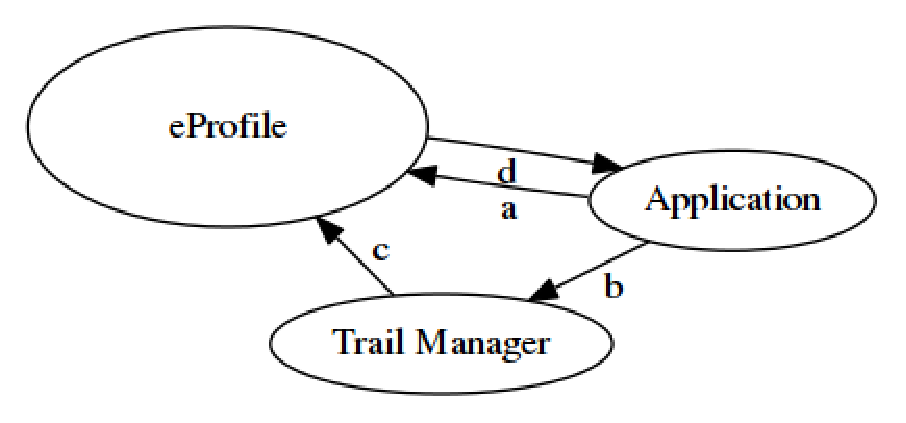
\includegraphics[width=0.6\textwidth]{modelobasico_en.eps}
  \caption{Overview of eProfile}
  \label{fig:modelobasico}
\end{figure}

Figure~\ref{fig:modelobasico} shows the overview of eProfile model, where each circle represents a component, and the arrows indicate the flow of data.

The {\bf application} is any piece of software that is being used directly by an entity. For an application to be considered suitable to use this model, it needs to record its information on a trail manager supported by eProfile. The application must also implement a communication protocol to exchange messages with eProfile. If these prerequisites are followed, the application can be of any type and run in any type of device that has communication with the Internet.

The second component depicted is a {\bf trail manager}. A trail manager is capable of storing events held by an entity, putting them in chronological order and registering information relevant to the event (e.g., the context in which the event was held). The eProfile supports any trail manager whose communication protocol is implemented in eProfile.

The third component of Figure~\ref{fig:modelobasico} represents the {\bf
eProfile}, where the arrows indicate the flow of data. The communication starts when the application registers itself on eProfile (arrow ``a''), sending (i) the entity model used by the application and (ii) the rules for construction of this model. From this moment on, the application starts recording the events on the trail manager (arrow ``b''). The eProfile periodically retrieves this information from the trail manager and builds or reconfigures the profile entity (arrow ``c''). When the application needs an updated profile, it retrieves this profile from eProfile (arrow ``d'').

Since eProfile supports multiple applications, it is possible for different applications to use different trail managers. Therefore, eProfile also supports communication with a number of trail managers, as exemplified in Figure~\ref{fig:gerenciadores}.

\begin{figure}
  \centering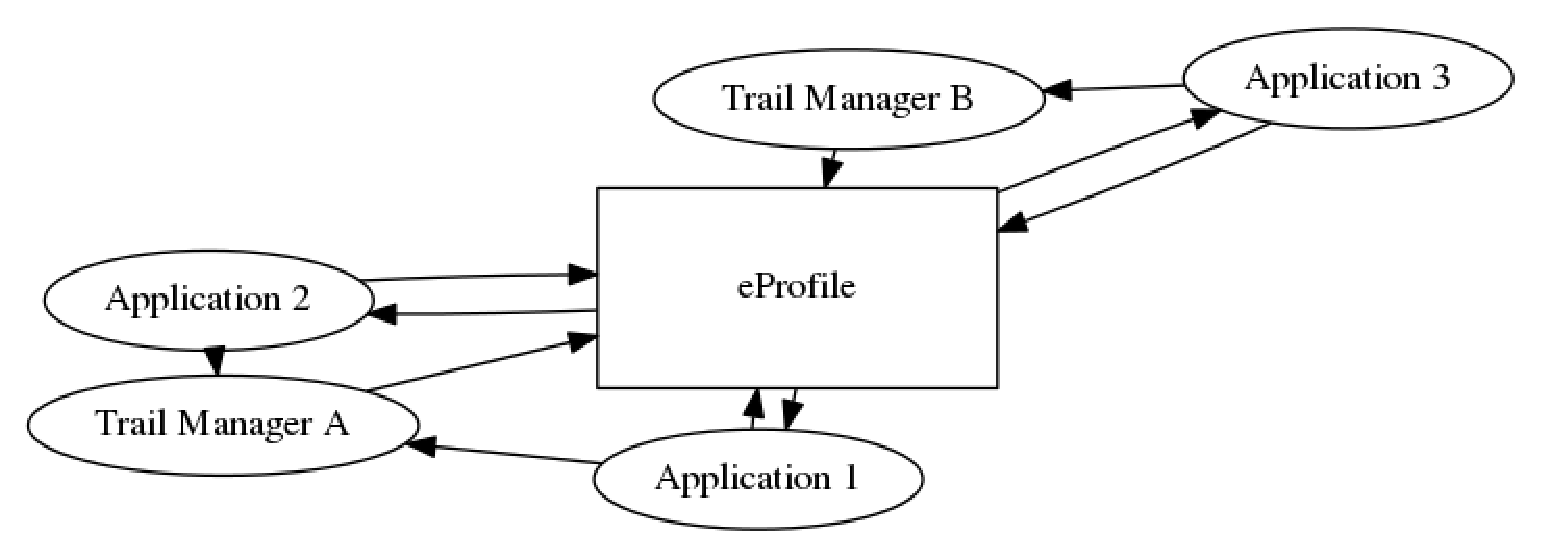
\includegraphics[width=1\textwidth]{modelo2_en.eps}
  \caption{eProfile connected to multiple trail managers}
  \label{fig:gerenciadores}
\end{figure}



%%%%%%%%%%%%%%%%%%%%%%%%%%%%%%%%%%%%%%%%%%%%%%%%%%%%%%%%%%%%



\subsection{Architecture}
\label{sec:arquitetura}

\begin{figure}
  \centering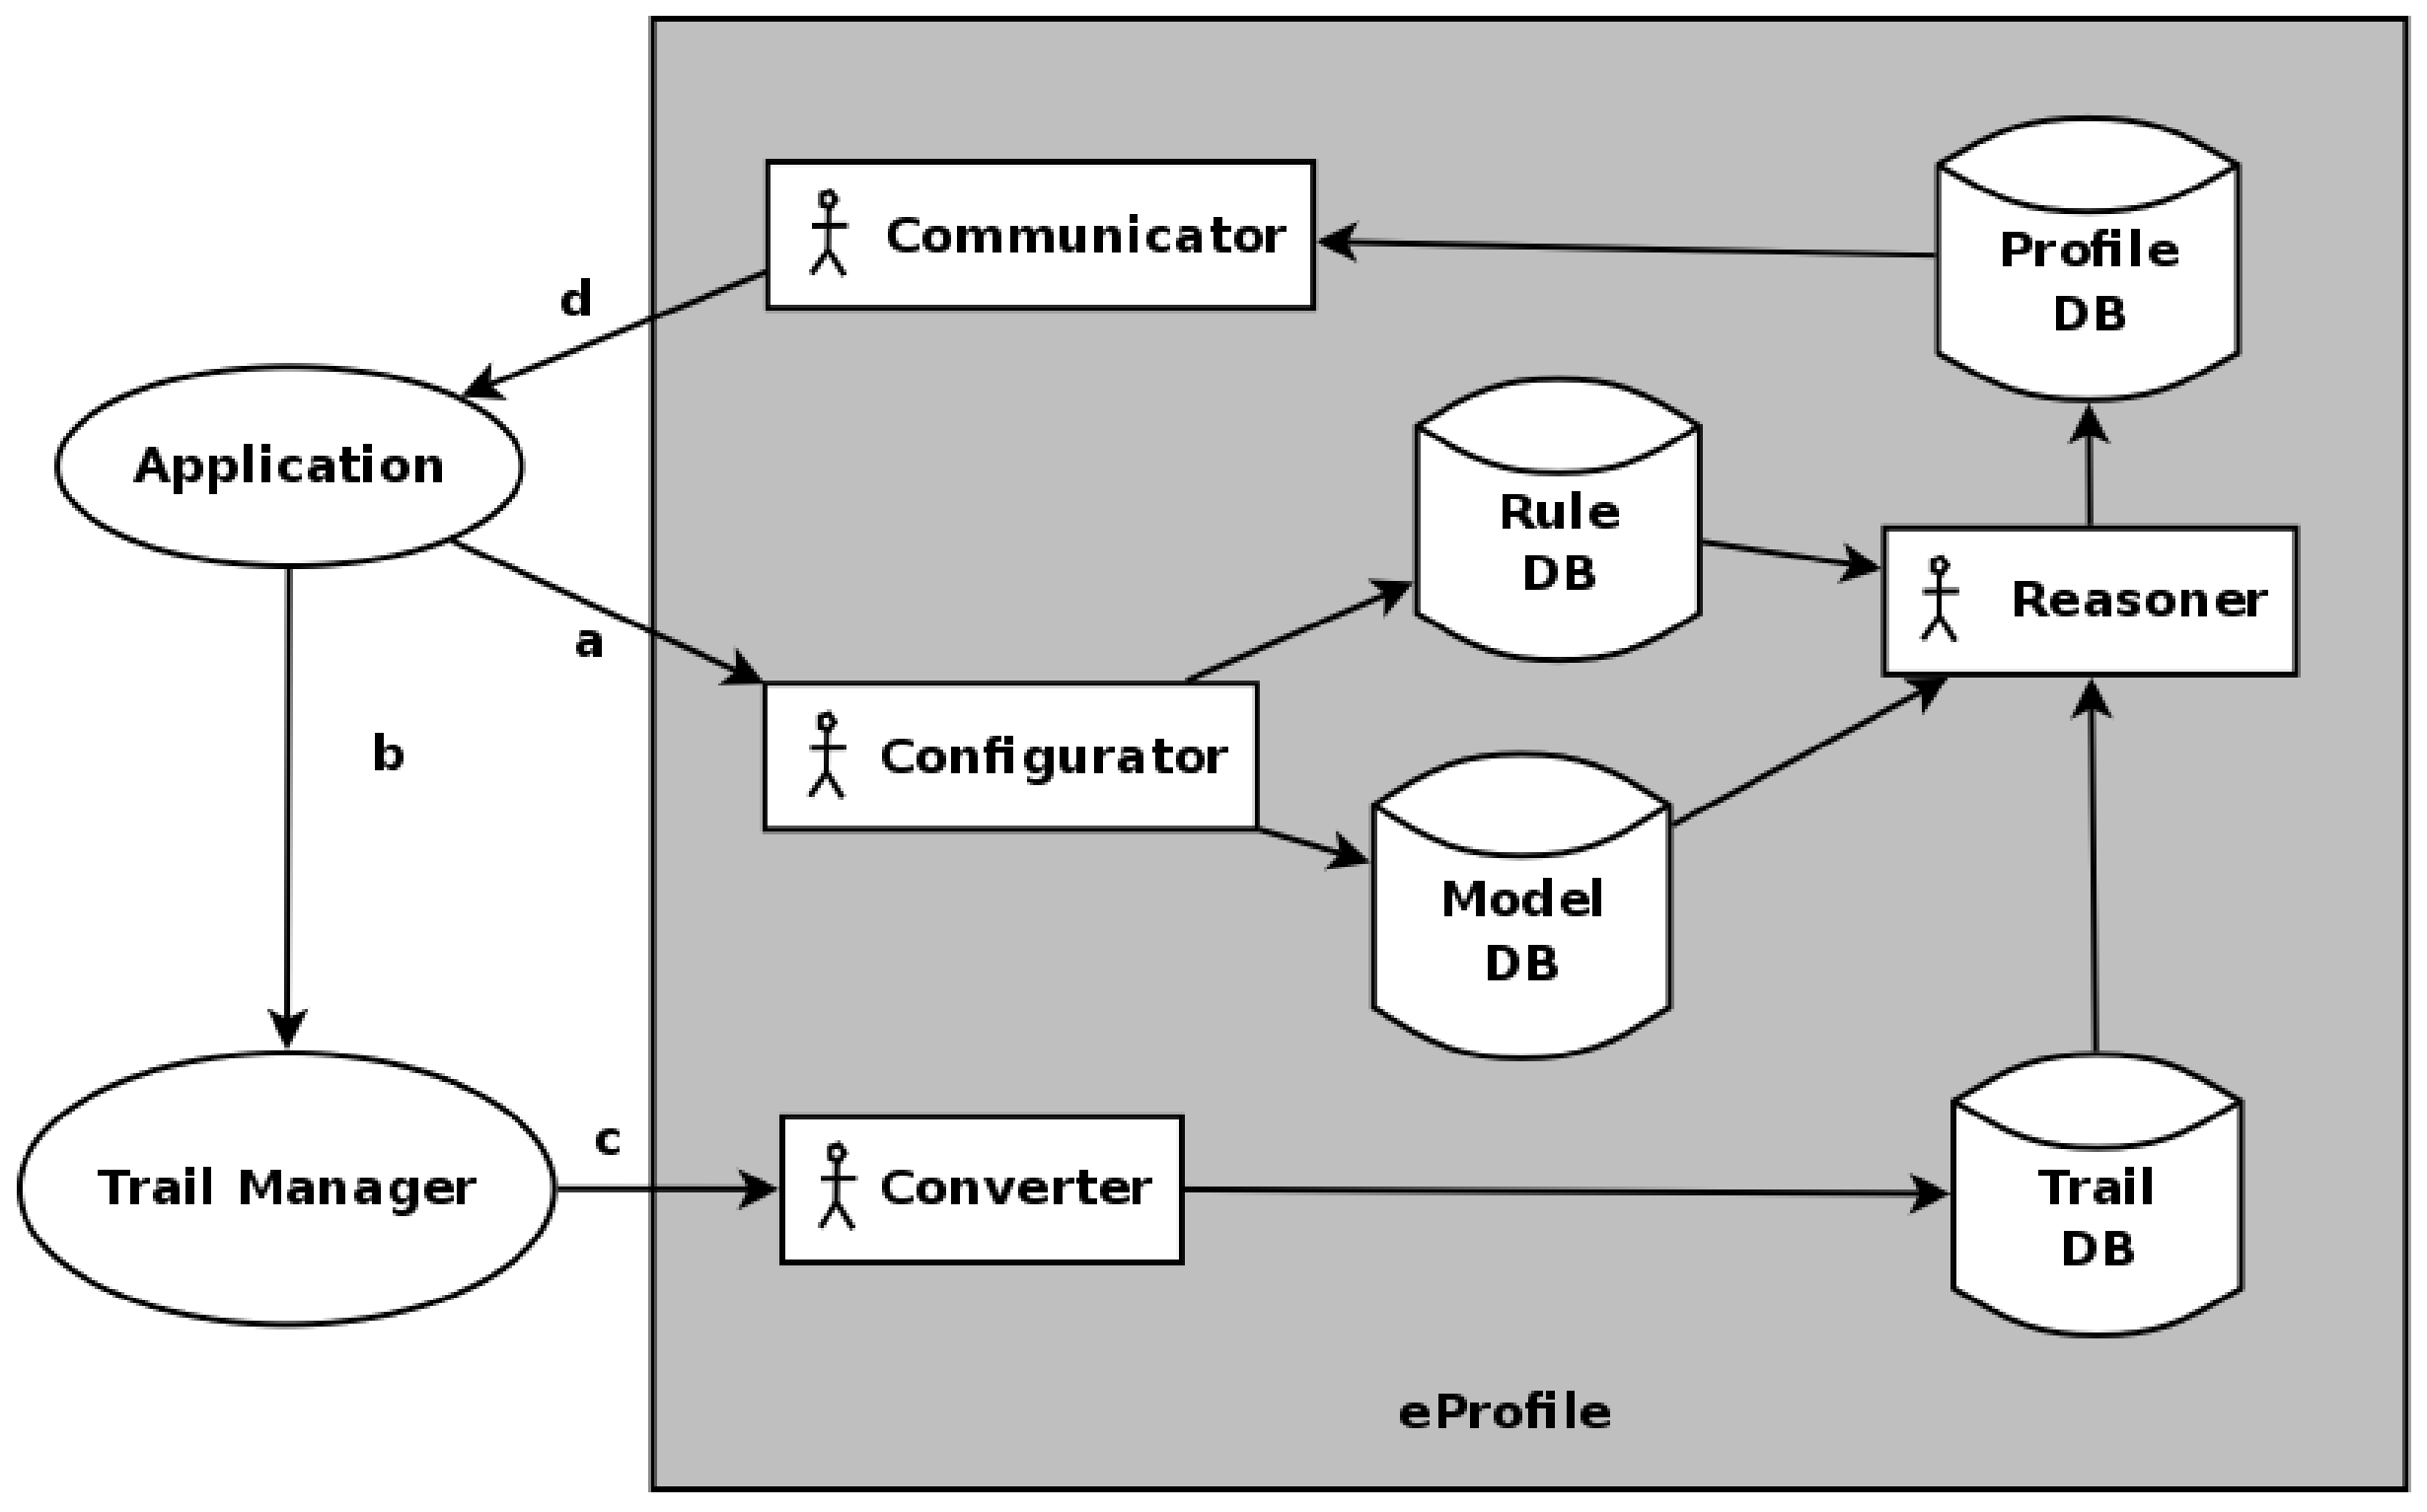
\includegraphics[width=1\textwidth]{modelo_big_en.eps}
  \caption{eProfile architecture}
  \label{fig:modelo}
\end{figure}

Figure~\ref{fig:modelo} shows the architecture of eProfile. The components ``Application'' and ``Trail Manager'' are the same as shown in Figure~\ref{fig:modelobasico}, while the ``eProfile'' was expanded to show its inner workings. The letters used in this figure represent the same ones used in Figure~\ref{fig:modelobasico}. The eProfile is composed by four autonomous agents and four databases. The usage of agents simplified the processing of ontology data and the inference execution.

%Since eProfile is a model that infers information about data stored in an ontology autonomously, and is organized into independent parts, it uses the technology of autonomous agents.

Each application builds its own entity model. The eProfile needs three pieces of information to be able to process the profiles: (i) the entity trail, (ii) the entity model used by the application and (iii) the inference rules for the profile. This can be seen in Figure~\ref{fig:modelo}, where the agent \textbf{Reasoner} receives data from these three databases. The trail of the entity is loaded by eProfile from the trail manager, while the other two information are sent directly from the application to eProfile. Thus, the inference rules defined by the application are used to infer the profile of the entity.

The arrows in Figure~\ref{fig:modelo} indicate the direction of the data flow, where it can be noted two entry points and one exit point.

The first entry point (arrow ``a'') is the information sent from the application to eProfile or, more specifically, to the {\bf Configurator} agent. The following information must be sent by the application:

\begin{itemize}

\item The entity model used by the application, which is the format of the entity profile. Once the entity trail is processed, the inferred data is stored and made available for application using this format;

\item  The rules used to infer the profile. These rules will be executed at
	regular intervals in order to update the entity profile. The
	Configurator receives the rules, validates them and inserts them in
	\textbf{rule database}. Along with the rules, is specified the
	criticality of information. The model uses this information to determine
	how often the profiles will be inferred.

\end{itemize}

The second entry point (arrow ``c'') allows receiving the entity trails, which are fetched by eProfile from the trail manager. Since eProfile can connect to different trail managers, (see Figure~\ref{fig:gerenciadores}), and each trail manager might use one specific format, a conversion between the original format and the format used by eProfile is needed for the trails to be stored in a standardized manner. This work is performed by an agent named {\bf Converter}, which is able to perform the conversion to the eProfile internal trail format.

The entity trail is then stored in a trail ontology called {\bf eOntoTrail}. This ontology contains the basic classes supporting the construction of a trail, and they can be extended according to the specification of the trail manager that is being used.

Once in possession of the trails, the model and rules, the \textbf{Reasoner} agent infers from the trail, generating a entity profile that consists of an extension of a basic profile ontology named {\bf eOntoProfile}. This ontology, just like the trail ontology, contains basic classes from which applications can specialize, using them to store their own information. The application can then connect to eProfile and get its entity profile, whose data are sent by the \textbf{Communicator} agent (arrow ``d'').


%%%%%%%%%%%%%%%%%%%%%%%%%%%%%%%%%%%%%%%%%%%%%%%%


\subsection{Ontologies}
\label{sec:ontologias}

As mentioned in Section~\ref{sec:arquitetura}, eProfile uses two ontologies: a trail ontology and a profile ontology. These are both basic ontologies, extended by sub-classes according to the trail format sent by the trail manager (for the trail ontology) or the needs of the application (for the profile ontology).

The trail ontology data (eOntoTrail), shown in Figure~\ref{fig:ont_trilha}, is fed by different trail managers. The Converter agent is responsible for receiving data in the trail manager format and converting it to the eOntoTrail. This way, the reasoner has a single ontology on which to reason.

\begin{figure}
  \centering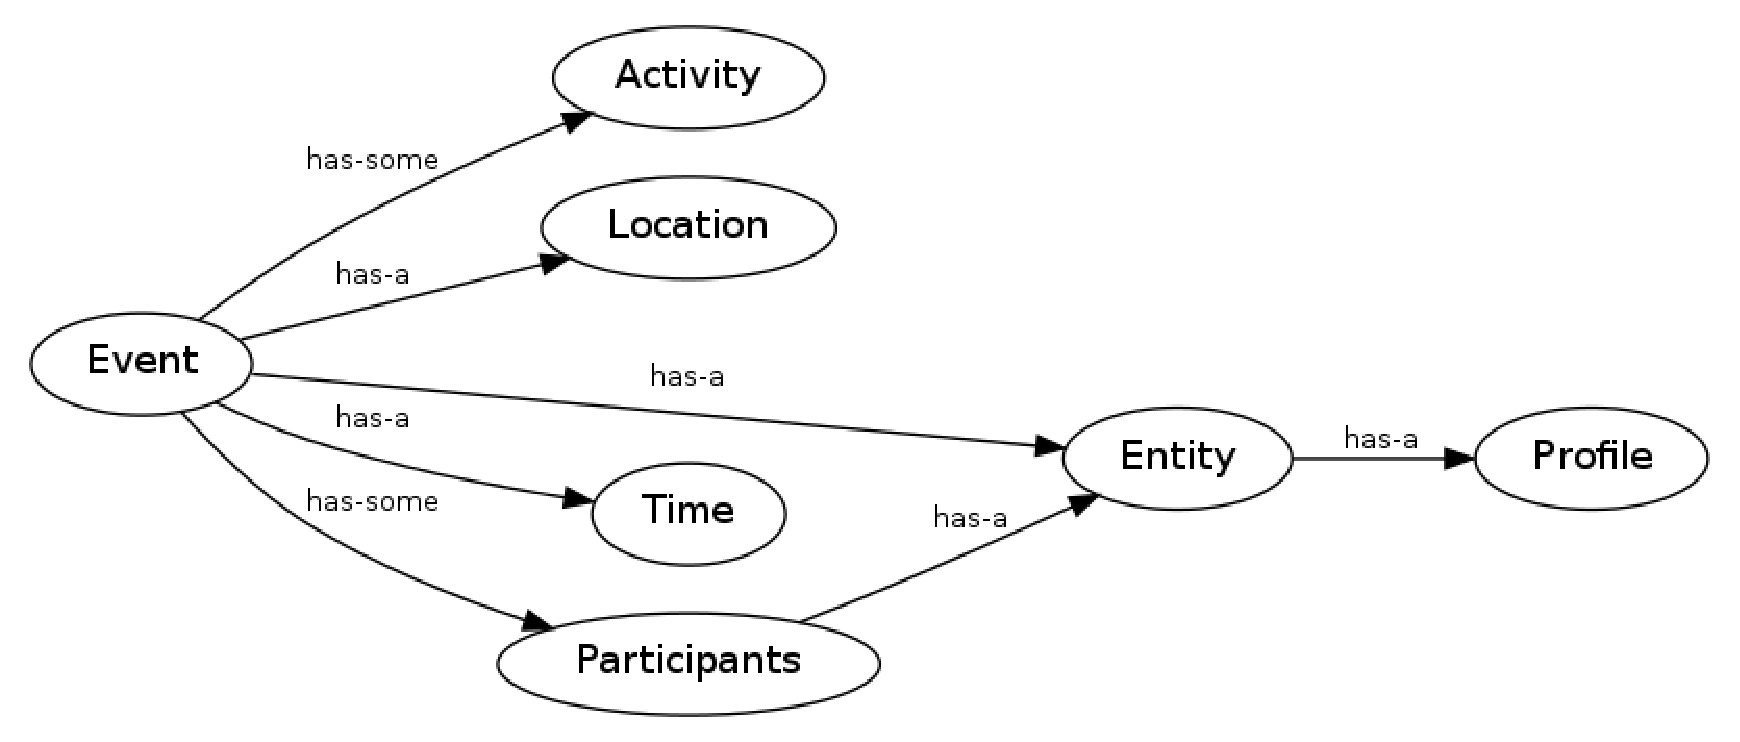
\includegraphics[width=1\textwidth]{ont_trilha_simples.eps}
  \caption{eProfile Trail Ontology (eOntoTrail)}
  \label{fig:ont_trilha}
\end{figure}

Context-aware applications are interested in knowing {\bf who}, {\bf where},
{\bf when} and {\bf what} (that is, what the user is doing), so they can
discover {\bf why} the situation is occurring \citep{abowd99}. Thus, a trail is
represented by a set of events characterized by the following main classes: (i)
{\em Entity}, the identity of the entity that is performing the action, which
can optionally be linked to a profile, (ii) {\em Location}, where the
action is taking place, (iii) {\em Time}, the date and time the event occurred,
(iv) {\em Participants}, the entities linked to this action, and (v) {\em
Activity}, the action that the entity is performing (or trying to perform). This
last class is the most comprehensive of the ontology, and will possibly be the most specialized by the trail managers.

\begin{figure}
  \centering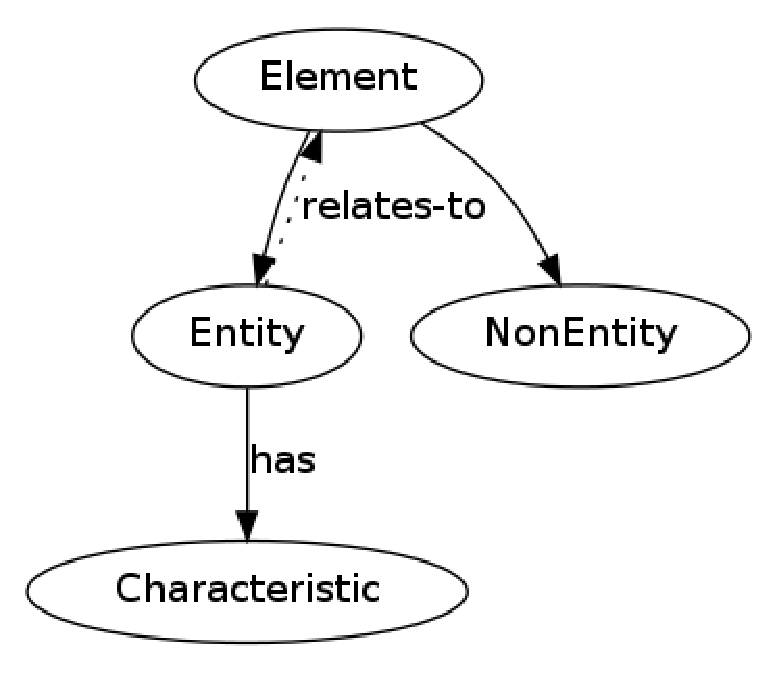
\includegraphics[width=0.45\textwidth]{ont_perfil3.eps}
  \caption{eProfile Profile Ontology (eOntoProfile)}
  \label{fig:ont_perfil}
\end{figure}

The profile ontology (eOntoProfile), shown in Figure~\ref{fig:ont_perfil}, is
the ontology used in the profile information inferred from the trail, according to the entity model defined by the application. For the ontology to be feasible within the proposed model, it must be a generic ontology that allows its classes to be extended by applications. In the figure, a relationship between classes is shown by a dotted line, and a specialization of a class is shown by a continuous line. The eOntoProfile is a basic ontology, extended by the applications to assemble their own entity models.

The basic class of the ontology is the {\em Element} class. This class represents anything in the real world. It is extended by two classes: (i) {\it Entity}, which represents an entity, that is, an element that has a profile associated with it, and (ii) {\it NonEntity}, which represents an element than doesn't have a profile associated with it. The class {\em Characteristic} represents an aspect of the entity, and is the class that will be extended by applications to refer to any information related to that entity. These characteristics can be simple labels (such as name of a person, or mileage of a car) or more complex information (such as academic knowledge or latest routes traveled).



\subsection{Rule Execution}
\label{sec:regras}

The execution of rules is key to eProfile's operation. An inference rule is an
instruction issued by an application, that runs on an entity trail, resulting in
an entity profile according to an entity model previously registered by the application.

For a rule to be executed, the application must have previously registered within eProfile: (i) the rule itself, (ii) an entity model, which serves as basis for the entity profile format, and (iii) the trail of the entity on which the inference is performed. From these three pieces of information, the reasoner is able to generate an entity profile, according to Figure~\ref{fig:dados_inferencia}.

\begin{figure}\centering
  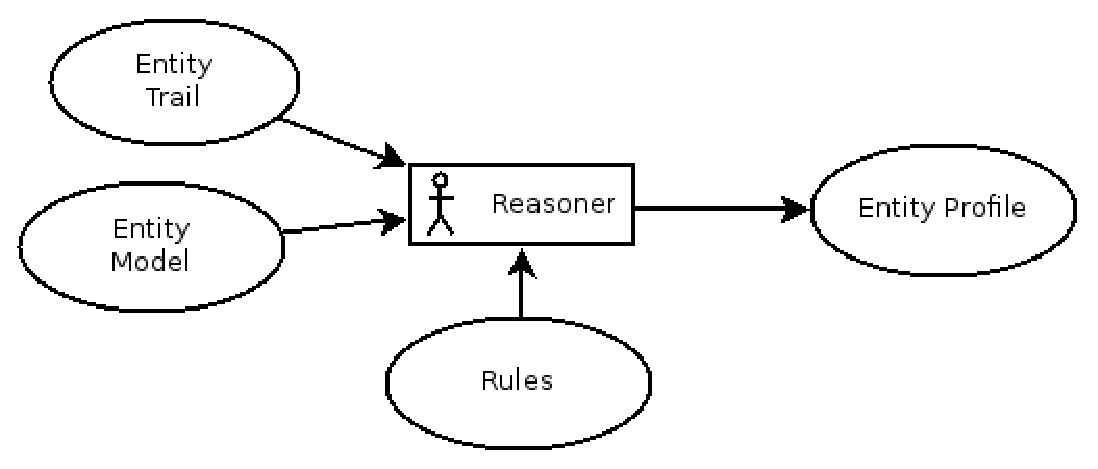
\includegraphics[width=0.9\textwidth]{dados_inferencia_en.eps}
  \caption{Data flow for the entity profile inference}
  \label{fig:dados_inferencia}
\end{figure}

The rules are always defined by the application, and a rule is composed of the
following set of information: (i) rule name, (ii) profile field that will be
updated, (iii) the rule, written in OWL language \citep{owl-guide}, (iv) update
method (replacement or update), (v) update frequency, and (vi) expiration of the rule.

The update method defines how the value will be changed in every execution of
the rule. There are two options: (i) replacement, where the value will be
replaced by a new information (for example, in the case of a person who changes
its address); and (ii) update, where the value is updated according with a
formula, that can take into consideration the current value (before the update).
The update option could be used, for example, in a field that stores the
interest of a person in a particular subject. The interest doesn't change
radically, but is changed smoothly based in the previously registered interest.

The update frequency defines how often the inference process will be executed, updating the profile. The expiration of the rule defines for how long a rule will be valid before it is deactivated.

The rules and the entity model can be changed at any moment during the execution
of eProfile. A change in the rules or in the model will reflect in a change in
the generated profile when the rules are executed the next time.

%-----------------------------------------------------------
\section{Implementation}
\label{ch:implementacao}

eProfile prototype was developed in Python \citep{python}. Python is a generic, open source, object-oriented, high-level language, that supports multiple architectures. % eProfile class diagram is represented in Figure~\ref{fig:classes}. The Communicator, Configurator, Converter and Reasoner classes implement the agents with the same names described in Section~\ref{sec:arquitetura}, and all of them inherit from class Agent, where the common agent tasks are implemented, such as setup, inter-agent communication and thread control.

%\begin{figure}
%  
\includegraphics[width=1\textwidth]{imagens/classes_en.eps}
%  \caption{eProfile class diagram}
%  \label{fig:classes}
%\end{figure}

The rule, model and profile information are stored in SQLite3 databases \citep{sqlite3}. SQLite3 is an SQL transactional self-contained database, available in the public domain. The SQLite3 was chosen due to its good performance and the fact that it does not require a separate server for deployment. The use of a relational database to store the rule, model and profile databases was made due to performance reasons.

% Figure~\ref{fig:dados_inferencia} shows the data flow for the entity profile
% inference process. 
The Reasoner agent uses an external inference engine to implement the rules. The reasoner used is FaCT++, a propositional logic reasoner created as a platform for use of algorithms of semantic {\em tableaux} and optimization techniques \citep{tsarkov06}. This reasoner was chosen due to its good performance and to support all functions used by eProfile. %The ConnectorFaCT class implements communication between the Reasoner agent and FaCT++ reasoner.

The knowledge representation language used for storage and processing of ontologies is OWL\citep {owl-guide}, chosen for being the most expressive ontology language defined for the Semantic Web \citep{daconta03}. Communication between eProfile, the trail managers and applications is done through REST web services \citep{fielding00}. %This intersystem connection is implemented in ConnectorWS class.

%%%%%%%%%%%%%%%%%%%%%%%%%%%%%%%%%%%%%%%%%%%%%%%%%%%%%%%%%%%%%%%%%%



\section{Evaluation Aspects}
\label{ch:cenario}

It is only possible to evaluate the functionalities of a proposed infrastructure by building applications that utilize it and then evaluate them, in order to obtain an indirect evaluation of the model \citep{edwards03}. The scientific community has been using scenarios to perform this type of indirect evaluation in context-aware (such as the approach taken by \citet{dey2001b}) and ubiquitous (according to \citet{satyanarayanan01}) environments. This work follows the same approach -- we created a prototype and a scenario for performing an experiment, in order to evaluate eProfile.

The application presented is based on the generation of simulated trails of undergraduate students within the context of Ubiquitous Learning. To build this application, eProfile was integrated with two softwares called LOCAL and UniManager. 

The following sections describe the applications used for the integration (Section~\ref{sec:cen1_apps}), the eProfile/LOCAL integration (Section~\ref{sec:eprofile_local}) and eProfile/UniManager integration (Section~\ref{sec:eprofile_unimanager}), the simulation environment (Section~\ref{sec:desc_cen1}), trails, rules and generated profiles (Section~\ref{sec:trilhas_cen1}) and the simulation parameters and results (Section~\ref{sec:simulacao_cen1}).

%%%%%%%%%%%%%%%%%%%%%%%%%%%%%%%%%%%%%%%%%%%%%%%%%%%%%%%%%%

\subsection{Applications}
\label{sec:cen1_apps}

\begin{figure}
  \centering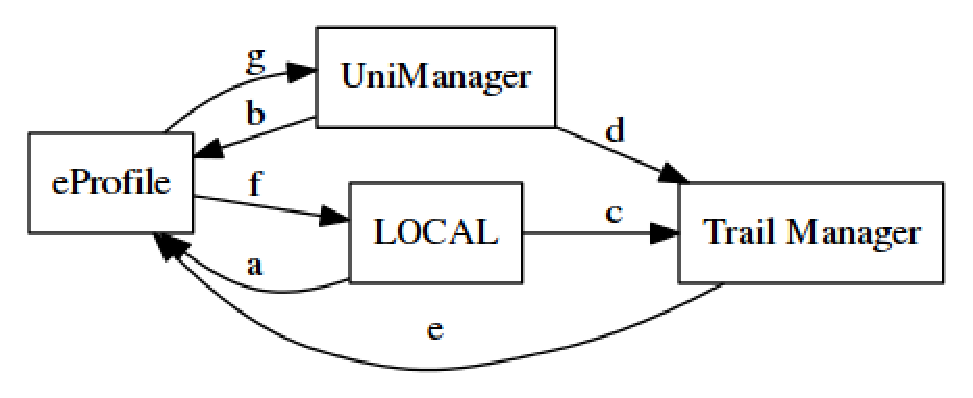
\includegraphics[width=0.6\textwidth]{modelo_cenario1_en.eps}
  \caption{Scenario model}
  \label{fig:modelo_cenario1}
\end{figure}

The integration is composed of four applications that interact among themselves, according to Figure~\ref{fig:modelo_cenario1}. LOCAL is a ubiquitous learning system used to find learning opportunities by putting students in touch and recommending learning content \citep{barbosa11}. UniManager is an application used by university administration to manage students grades and disciplines. 

Both LOCAL and UniManager have profile modules, and the profile information is used for making decisions. Since in both cases the profile module is static and depends on collection of explicit information, eProfile is connected to these softwares, leveraging the dynamic creation of profiles and collecting information implicitly. Furthermore, eProfile enables interoperability between these systems by allowing information from both systems to be used to generate single profiles. The scenario also includes a trail manager, that manages the entities trails. In this scenario, the disciplines and students are represented as entities.

The initial communication occurs between applications and eProfile (arrows ``a'' and ``b''), where applications define their entity models and rules. This data exchange can occur as often as necessary, because applications can update their rules and their entity models at any time. During the execution of the applications, they record the events in the trail manager (arrows ``c'' and ``d''). This means that applications can run disconnected from eProfile, and connect only when a rule needs to be updated or when profile data must be downloaded. eProfile retrieves trails periodically from the trail manager (arrow ``e''). When eProfile is in possession of the trails, rules and entity models, it starts to process this information, inferring new profile data. These profiles are then downloaded by the applications (arrows ``f'' and ``g'').

%%%%%%%%%%%%%%%%%%%%%%%%%%%%%%%%%%%%%%%%%%%%%%%%%%%%%%%

\subsection{eProfile/LOCAL Integration}
\label{sec:eprofile_local}

This scenario integrates eProfile to a ubiquitous learning system called LOCAL (Location and Context-Aware Learning). LOCAL uses location information and context as an aid to teaching and learning process. A location system monitors the mobility of apprentices and, based on their physical position, explores educational opportunities \citep{barbosa11}.

\begin{figure}[!t]
  \centering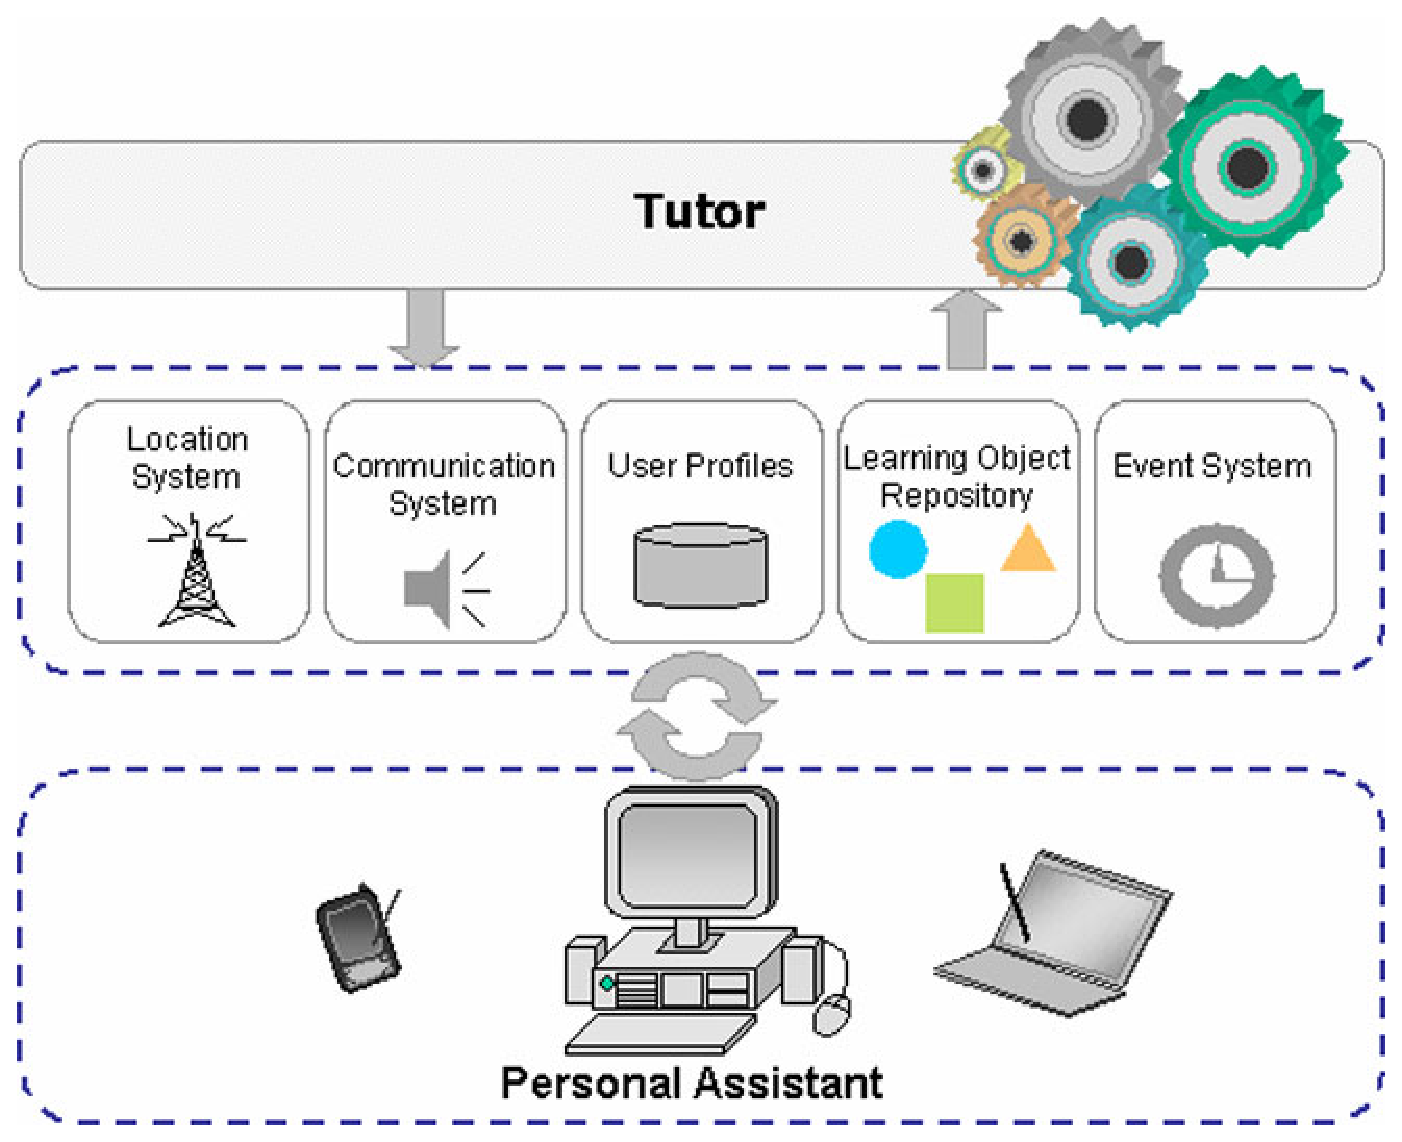
\includegraphics[width=0.7\textwidth]{arq_local.eps}
  \caption{LOCAL model \citep{barbosa11}}
  \label{fig:arq_local}
\end{figure}

LOCAL architecture is shown in Figure~\ref{fig:arq_local}. The gathering of LOCAL's profile system information is explicit. This means that users' (learners) relevant data need to be pre-populated in the system. Furthermore, the LOCAL profile system is static, which means that data is not automatically updated in response to actions taken by learners or external events. Since eProfile is a dynamic entity model with implicit information collection, integrating these two models result in the enhancement of LOCAL capabilities.

LOCAL and eProfile integrate according to Figure~\ref{fig:eprofile_local}. Besides LOCAL and eProfile, Figure~\ref{fig:eprofile_local} presents an application called Trail Manager. The Trail Manager is an external program that stores the trails, processes them and forwards them to eProfile, as described in Section~\ref{ch:modelo}. For this scenario, we created a simple trail manager, which just receives, stores and forwards the trails to eProfile upon request.

Integration between eProfile and LOCAL was based on the following changes to
LOCAL: (i) we included a connection interface with eProfile, able to generate
learners entity models and rules for profile processing, (ii) we included a
connection interface with the trail manager, to allow the location events and
actions undertaken on the Personal Assistant to be sent to the trail manager,
and (iii) we included a communication interface with eProfile, where the LOCAL
User Profiles module is fed by profiles generated by eProfile.

\begin{figure}[!t]
  \centering\includegraphics[width=1\textwidth]{eprofile_local_en.eps}
  \caption{eProfile/LOCAL Integration}
  \label{fig:eprofile_local}
\end{figure}

As learners use LOCAL, their location changes are identified by the Location
System component, and their actions are done on the Personal Assistant. These
components record events in the Trail Manager (arrows ``b'' and ``c''), which in
turn sends them to the Converter eProfile agent (arrow ``d''). Trails sent are
stored in the Trail database. These trails are periodically processed according
to the models and rules defined initially, and a inference process based on this
information generates profiles, which are sent to the LOCAL User Profiles module
(arrow ``e'') by the Communicator agent. These profiles help LOCAL to know its
users (learners) in order to put them in contact and distribute content in the most contextualized possible way.


% - Contato: seria gerado a partir das informações básicas dos alunos.
%Por exemplo, o aluno registra seu nome, esta informação entra na
%trilha e daí vai para o perfil.
% - Preferências: ?
% - Interesses: gerado a partir das escolhas do aluno, que descrevi no ponto 3;
% - Relacionamentos: gerado principalmente a partir as informações do
%Gerenciador de Disciplinas;
% - Desempenho: gerado a partir das notas dos alunos;
% - Segurança: acredito que não seja relevante para o cenário.


% TODO - formação de perfil do LOCAL

%%%%%%%%%%%%%%%%%%%%%%%%%%%%%%%%%%%%%%%%%%%%%%%%%%%%%%%%%

\subsection{eProfile/UniManager integration}
\label{sec:eprofile_unimanager}

UniManager is a administrative software used by the university for registration and management of students and disciplines. This application model is shown in Figure~\ref{fig:unimanager}.

\begin{figure}[!t]
  \centering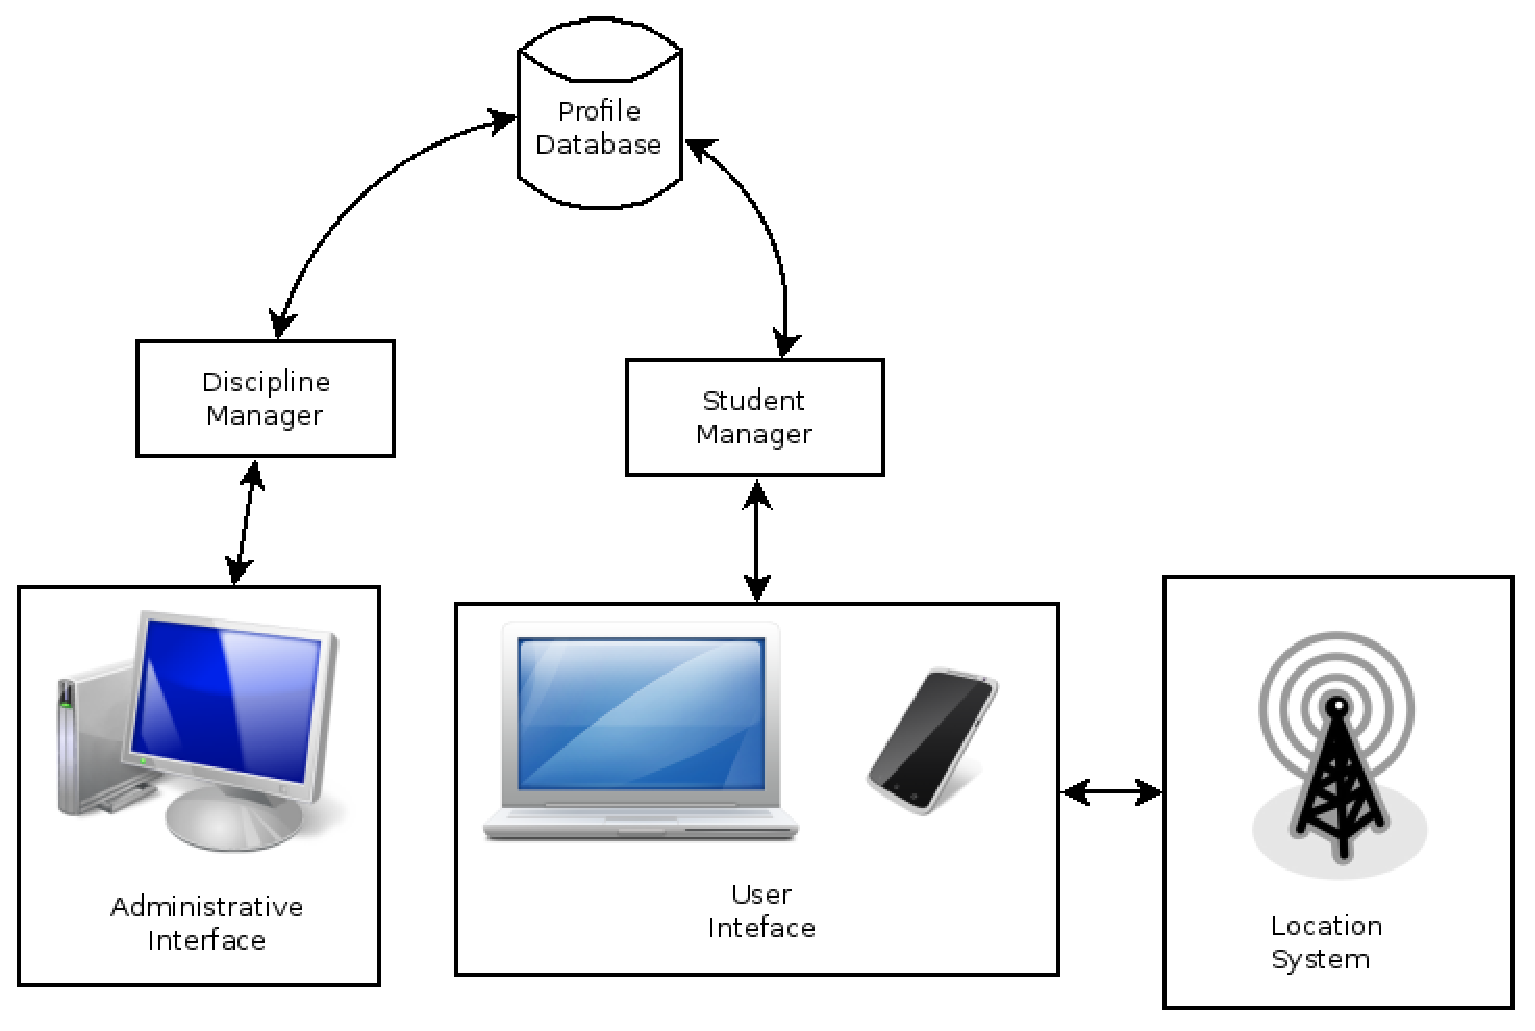
\includegraphics[width=0.9\textwidth]{unimanager_en.eps}
  \caption{UniManager model}
  \label{fig:unimanager}
\end{figure}

UniManager has two interfaces: administrative and user. The administrative interface is used by the management of the university to enroll disciplines and students. It is also used by students to carry out their registration for the next semester. This interface connects to a discipline manager, which manages the enrollment and prerequisites between disciplines.

The user interface is used in the students' mobile devices, and
is connected to the university location system. Thus, all events recorded in
UniManager from this interface contains the location of the student within the
university, that is, the campus' region where the student is. The location system integrated to the user interface allows the system to check whether the student is present in class. The student performs the tests and hands out papers using this interface.

UniManager also contains a profile database. On this database are stored: (i) registration information about the disciplines, (ii) presences and absences of students, (iii) tests and papers handed out by the students, and (iv) the evaluation of student work.

The profile database is dynamically updated based on recorded events, but is limited to data recorded in UniManager itself. Integration between eProfile and UniManager leverages the generation of more advanced profiles, using the information inferred by eProfile from the data generated by LOCAL. Using this data, it is possible to register the interests of the student in UniManager's profile database, in order to suggest him optional subjects that might be of his interest. Furthermore, the use of trails allows the profiles to be generated based on historical information. 

\begin{figure}[!t]
  \centering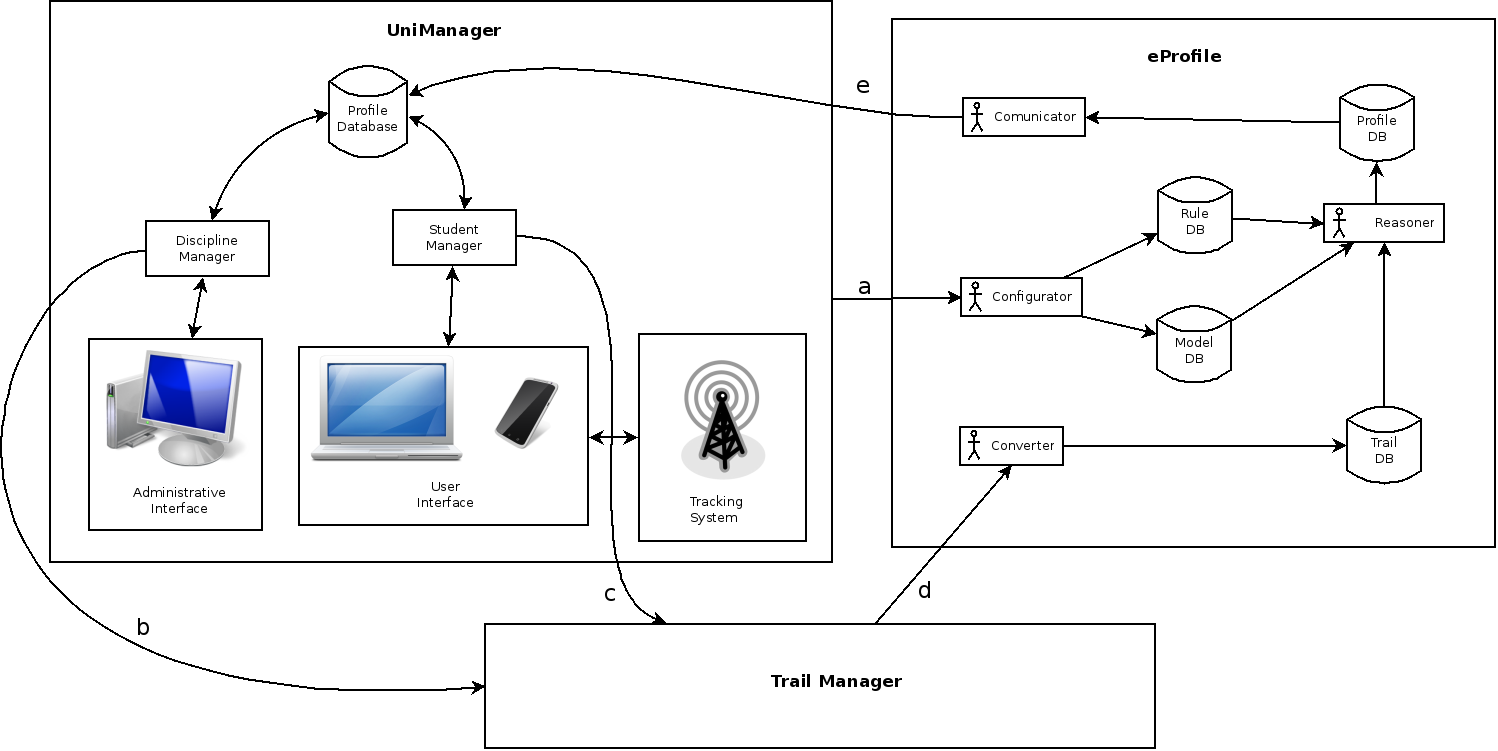
\includegraphics[width=1\textwidth]{unimanager_eprofile_en.eps}
  \caption{UniManager/eProfile integration}
  \label{fig:unimanager_eprofile}
\end{figure}

UniManager integrates to eProfile according to Figure~\ref{fig:unimanager_eprofile}. In the first communication between UniManager and eProfile,  UniManager sends messages indicating to eProfile which are the entity models and the rules used to generate the profiles (arrow ``a'').  This information is received by the Configurator agent, responsible for validating and storing the rules and models in their respective databases. As users make use of the UniManager interfaces, data is processed and stored by the Discipline and Student Manager modules in the trail manager, along with their location (arrows ``b'' and ``c''). The trail manager used by UniManager is the same one used by LOCAL. The trail manager periodically sends the trails generated by UniManager to the Converter agent in eProfile (arrow ``d''). This agent converts the trails to the eProfile format and stores them in the trail database. Once in possession of the trails, models and rules, the Reasoner agent processes the information and generates profiles that are sent to UniManager by the Communicator agent (arrow ``e''). 

%%%%%%%%%%%%%%%%%%%%%%%%%%%%%%%%%%%%%%%%%%%%%%%%%%%%%%%%%

\subsection{Environment}
\label{sec:desc_cen1}

The scenario consists of a group of students that carries out a graduation course in Computer Science. The course consists of a total of 40 disciplines, of which 12 are optional (the student must complete at least 8 out of these 12). All disciplines have other disciplines as prerequisites, except for the disciplines of the beginning of the course.

Students use mobile devices (laptops or smartphones), on which the applications used for administration of their academic life are installed -- in particular, UniManager and LOCAL.

UniManager is the system used for discipline administration, and it is described in detail in Section~\ref{sec:eprofile_unimanager}. It is used by the university administration and the students. The administration uses it to register disciplines, and students, to link students to their disciplines and to issue management reports such as attendance and approval/failing of students. Students use it to hand out their tests and papers, to make their enrollment in the disciplines and to check their grades and absences.

In addition, professors and students also use LOCAL on their mobile devices. LOCAL is described in more detail in Section~\ref{sec:eprofile_local} and in \citep{barbosa11}. LOCAL links profile information with the user location, facilitating interaction between learners and enabling the delivery of contextualized educational material. Professors use the LOCAL to register material that will be distributed to students. LOCAL communicates with students to distribute educational material previously registered and to put students with similar interests in touch during educational activities. If, during these activities, the student has not registered any interest that matches those required by the activity, he has the option to make the choice using a user interface to LOCAL called Personal Assistant.

Table~\ref{tab:aula} exemplifies a two and a half hours class involving 10 students, in which there was a debate about Programming Techniques. After the debate, students undertook a study about the individual topics discussed in the debate. In this example, the presence of students, the handing out of their work and the grade achieved were registered in UniManager. The educational content of the lesson was registered in LOCAL.

In this example, LOCAL registered the personal preferences of two students about programming techniques. If LOCAL and UniManager were being used in isolation, this information would have been relevant only to the immediate lesson assignment. However, the integration of these systems with eProfile allows this information to be used to update the profile of the students, and can be used in the future to facilitate interaction between students and personalize the delivery of educational content (by LOCAL). Furthermore, a single profile can be generated by the trails from both applications, this information can be used to assist the student in the recommendation of optional disciplines (by UniManager).

\begin{table*}\centering\footnotesize
    \begin{tabular*}{1\textwidth}{@{}cccp{6.8cm}@{}}
    \toprule
    Event & Time & Actor & Action \\
    \midrule
    1 & - & Professor & Registers educational material that will be used in
class into LOCAL, and requests the handing out of a paper through UniManager. \\
    2 & 7:30 & Students & Nine students enter the classroom. \\
    3 & 7:30 & LOCAL & LOCAL identifies the entrance of the students into the classroom. \\
    4 & 7:30 & UniManager & UniManager identifies the entrance of the students into the classroom. \\
    5 & 7:30 & LOCAL & LOCAL sends the class educational material to the students. \\
    6 & 8:00 & Professor & The professor requests the formation of groups for the debate. \\
    7 & 8:00 & LOCAL & LOCAL forms three groups based on the students' preferences: {\em Distributed Algorithms} (3 students), {\em Scheduling Algorithms} (3 students) and {\em Math Algorithms} (1 student). Two students have no registered preference that would allow LOCAL to put them in some group. \\
    8 & 8:00 & LOCAL & LOCAL request the two students to choose a group. \\
    9 & 8:10 & Students & Students indicate their preference through LOCAL Personal Assistant. \\
    10 & 8:10 & LOCAL & LOCAL puts the two students in their chosen groups, one of them in {\em Scheduling Algorithms} and the other one in {\em Math Algorithms}. \\
    11 & 8:10 & Students & The debate starts. \\
    12 & 8:40 & Students & One student enters the classroom, late. UniManager and LOCAL register his entrance, but LOCAL doesn't integrate him in the debate, since it's almost over.\\
    13 & 8:50 & Students & The debate ends. \\
    14 & 8:50 & Professor & The professor request the students to write a paper about the debate subject.\\
    15 & 10:00 & Students & The students hand out their papers through UniManager and leave the classroom.\\
    16 & 10:00 & UniManager & UniManager receives the papers and registers the students exit.\\
    17 & 10:00 & LOCAL & LOCAL registers the students exit.\\
    18 & - & Professor & The professor, later, evaluates the students papers and registers their grades on UniManager.\\
    \bottomrule
  \end{tabular*}
  \caption{Example of a class}
  \label{tab:aula}
\end{table*}

%%%%%%%%%%%%%%%%%%%%%%%%%%%%%%%%%%%%%%%%%%%%%%%%%%%%


\subsection{Trails, Rules and Profiles}
\label{sec:trilhas_cen1}

According to what was described in Sections~\ref{sec:eprofile_local} and \ref{sec:eprofile_unimanager}, LOCAL and UniManager suffered three significant changes: (i) there were included communication interfaces with eProfile, so that applications can provide the entity models and rules, (ii) there were included  communication interfaces with the trail manager, so that applications could register the events and (iii) the profile modules of both applications were modified to request profile updates from eProfile.

The scenario consists of two types of entities: students and disciplines. The ``student'' entities represent each one of the students involved in the course. The ``discipline'' entity refers to each discipline of the course. A discipline could be represented either as an entity or as a single resource; in this scenario, we decided that it would be represented as an entity, since this  allows it to create a trail, from which a profile can be obtained. This way, the profile of the discipline can contain fields that are updated automatically such as, for example, the average grade of the discipline.

%According to the description in Section~\ref{sec:arquitetura}, context-aware applications are interested in knowing {\bf who}, {\bf where}, {\bf when} and {\bf what} (ie, what the user is doing), so they can understand {\bf why} the situation is occurring. The eProfile trail ontology, shown in Figure~\ref{fig:ont_trilha}, defines that these questions are answered, respectively, by the classes {\em Entity}, {\em Location}, {\em Time} and {\em Activity}. Furthermore, the class {\em Participants} describes the other entities involved in this event. When a trail is stored in eProfile, information regarding the event should be inherited from these classes, using as many classes as necessary so that the information is complete.

%The students' trail, as registered by LOCAL and UniManager, contains the following kind of events: registration, discipline enrollment, entry and exit from locations inside the campus, handing out of test and papers, new preferences and abandonment of the course. The trail format is detailed in Figure~\ref{fig:ont_estudante}. The following events are registered in the professor trail: registration, entry and exit from locations inside the campus and evaluation of students' tests and papers, according to the diagram shown in Figure~\ref{fig:ont_docente}. The discipline trail receives the following events: registration, beginning and end of semester and work group, according to Figure~\ref{fig:ont_disciplina}.

%\begin{figure}[!t]
%  \centering
\includegraphics[width=0.6\textwidth]{imagens/ont_estudante.eps}
%  \caption{Student trail ontology}
%  \label{fig:ont_estudante}
%\end{figure}

%\begin{figure}[!t]
%  \centering
\includegraphics[width=0.6\textwidth]{imagens/ont_docente.eps}
%  \caption{Professor trail ontology}
%  \label{fig:ont_docente}
%\end{figure}

%\begin{figure}[!t]
%  \centering
\includegraphics[width=0.6\textwidth]{imagens/ont_disciplina.eps}
%  \caption{Discipline trail ontology}
%  \label{fig:ont_disciplina}
%\end{figure}

%The ultimate goal of trail inference is the profile generation. For eProfile to be successful in generating profiles from trails, it requires the application to inform the entity models and the inference rules.

%The entities models are the data structure used to store the profile of a entity. The entity model used by the LOCAL User Profile module is shown in Figure~\ref{fig:perfil_local}. The learners' profiles have two types of data: (i) persistent, associated to the learner in any situation, and (ii) contextual, associated with which the contexts in which the learner interacts.

%\begin{figure}[!t]
%  \centering
\includegraphics[width=0.7\textwidth]{imagens/perfil_local.eps}
%  \caption{LOCAL profile model \citep{barbosa11}}
%  \label{fig:perfil_local}
%\end{figure}

%Sections of the profile persistent block are (i) contact, which stores basic information of the user (such as name, phone number, among others), (ii) preferences, which stores the media type preferred by the user, and (iii) interests, which identifies the student's topics of interest. The interests section is categorized according to ACM's computational classification system \citep{acm10}. Sections of the contextual block are (i) relations, identifying relationships with other users within the same context, (ii) performance, which refers to the goals to be achieved by students and (iii) security, which stores credentials necessary to access different levels in specific contexts.

%UniManager stores profiles of disciplines, professors and students. Its entity model is illustrated in Figure~\ref{fig:perfil_unimanager}. The basic information, disciplines enrolled and notes/absences from the student profile, along with the disciplines information, are used for managerial activities of the university, such as checking if the student can attend a particular discipline. Performance information about the professor and historical average grades of disciplines are used to adjust the professor with the discipline he has higher affinity or performance. Information about students interests are used to suggest optional disciplines to them.

%\begin{figure}[!t]
%  \centering
\includegraphics[width=0.65\textwidth]{imagens/unimanager_perfil_en.eps}
%  \caption{UniManager profile model}
%  \label{fig:perfil_unimanager}
%\end{figure}

%Each application defines a set of rules for profile generation based on the trails registered by each one. An application has the option of using the trail of another application for processing rules and, consequently, profile generation, thus allowing the entity profile to be enriched by the surrounding environment.

%The rule definition is written in OWL by creating classes that can be processed by a reasoner. Table~\ref{tab:aula} shows an example of a classroom where the professor registers in LOCAL a set of subjects that will be discussed in class (event 1). This event generates a trail that is sent from LOCAL to the trail manager and, subsequently, to eProfile.

%LOCAL then tries to identify students who have the same interests as the ones in the proposed debate, or interests related to these (event 7), by sending the OWL rules described in Figure~\ref{fig:regra1}. The first rule is called {\em RelatedSubjects} (line 2), where the subjects (class {\em Subject}, in line 4) related (line 6) to what will be discussed in class (line 7) are inferred. The expression {\tt ?Subject} is an eProfile extension to OWL, where this expression is replaced by the subjects that will be discussed, allowing the same rule to be used in different situations. This rule, after the inference process, results in the listing of all subjects (classes of type {\em Subject}) that relate to the subject that will be discussed, putting these classes as sub-classes of class {\em RelatedSubjects}.

%Using this rule, it is possible to find out the students (line 15) whose interests intersect with the interests found in the {\em RelatedSubjects} class (line 18). These students, in this ontology, become sub-classes of class {\em StudentsSelected} (line 13).

%\begin{figure}[!t]
%\begin{verbatim}
% 1  <EquivalentClasses>
% 2    <Class IRI="RelatedSubjects"/>
% 3    <ObjectIntersectionOf>
% 4      <Class IRI="Subject"/>
% 5      <ObjectSomeValuesFrom>
% 6        <ObjectProperty IRI="isRelated"/>
% 7        <Class IRI="?subject"/>
% 8      </ObjectSomeValuesFrom>
% 9    </ObjectIntersectionOf>
%10  </EquivalentClasses>
%11
%12  <EquivalentClasses>
%13    <Class IRI="StudentsSelected"/>
%14    <ObjectIntersectionOf>
%15      <Class IRI="Student"/>
%16      <ObjectSomeValuesFrom>
%17        <ObjectProperty IRI="hasInterest"/>
%18        <Class IRI="RelatedSubjects"/>
%19      </ObjectSomeValuesFrom>
%20    </ObjectIntersectionOf>
%21  </EquivalentClasses>
%\end{verbatim}
%  \caption{OWL rule for identification of students interests}
%  \label{fig:regra1}
%\end{figure}

%Event 7 in Table~\ref{tab:aula} describes that two students did not match either group because they had no interest related to the subjects of debate, and LOCAL asked them on what subject they would like to participate (events 8 and 9), thus generating a trail event for these two students. Once the trail is registered, the student's profile is reprocessed according to the rules defined by LOCAL.

%The header of the rule that updates the student interest field is shown in Figure~\ref{fig:regra3}. This header defines that the student profile (line 1) {\em Interest} field (line 2) will be updated using the sub-classes of class {\em StudentInterest}, whose OWL rule is shown in Figure~\ref{fig:regra2}. It is also defined that a new interest is added to the interests that already exist (line 4), that this rule is updated every time an event is registered in the trail in which a subject is chosen (line 5). The OWL rule of Figure~\ref{fig:regra2} defines that the {\em StudentInterest} class consists of the subjects chosen (line 6) by the students who are part of this context (line 10 and 11) and that have chosen a particular subject (lines 6 and 7).

%\begin{figure}[!t]
%\begin{verbatim}
%1  Profile:   Student
%2  Field:     Interest
%3  Rule:      StudentInterest
%4  Update:    addition
%5  Frequency: onTrailEvent(SubjectChosen)
%6  Expires:   never
%\end{verbatim}
%  \caption{Student profile rule header}
%  \label{fig:regra3}
%\end{figure}

%\begin{figure}[!t]
%\begin{verbatim}
% 1  <EquivalentClasses>
% 2    <Class IRI="StudentInterest"/>
% 3    <ObjectIntersectionOf>
% 4      <Class IRI="SubjectChosen"/>
% 5      <ObjectSomeValuesFrom>
% 6        <ObjectProperty IRI="subjectChosen"/>
% 7        <Class IRI="Subject"/>
% 8      </ObjectSomeValuesFrom>
% 9      <ObjectSomeValuesFrom>
%10        <ObjectProperty IRI="hasStudent"/>
%11        <Class IRI="?student"/>
%12      </ObjectSomeValuesFrom>
%13    </ObjectIntersectionOf>
%14  </EquivalentClasses>
%\end{verbatim}
%  \caption{Student profile OWL rule}
%  \label{fig:regra2}
%\end{figure}

%After the execution of the rule shown in Figures~\ref{fig:regra3} and~\ref{fig:regra2}, the rule in Figure~\ref{fig:regra1} runs again, this time identifying students who made their choice (event 10 of Table~\ref{tab:aula}).

%%%%%%%%%%%%%%%%%%%%%%%%%%%%%%%%%%%%%%%%%

\subsection{Prototype and Simulation}
\label{sec:simulacao_cen1}

The scenario objective was to evaluate the integration between eProfile, LOCAL and UniManager through a four year undergraduation course, which made a real-life scenario impractical. A simulation was thus created to validate the model. Two programs were developed:

\begin{enumerate}
  \item A simulator, which simulates students, professors and disciplines using UniManager and LOCAL;
  \item A trail manager, which stores the generated trails and makes them available to eProfile.
\end{enumerate}

To simulate the scenario as faithfully as possible, each entity was created with a set of characteristics that distinguish them from one another, and causes them to have different performances and take different decisions when faced with a choice. These characteristics directly influence the quality of student learning, the difficulty of the course and the likelihood of dropout students. Students are generated with varying levels of commitment, intelligence and personal tastes. These characteristics influence student performance, the probability of withdrawal of disciplines and course, and the choices that the student will make.

The scenario simulates a group of 40 students who conduct a course in Computer Science at a university. A simulation starts with the creation of the discipline and student entities. The initial profiles of the disciplines are then generated. A loop then start, and it will only end when all students have completed the course or dropped out. Each iteration of the loop is a semester course and contains the following steps:

\begin{enumerate}
\item Students choose the disciplines they will attend and enroll;
\item Each day of the course is simulated, where students attend class and perform tests or deliver papers;
\item The students final grades are calculated, and the students decide if they will continue on the course or drop out.
\end{enumerate}

Each course consists of 14 classes. There are two types of events that can occur in a class: (i) a debate or group work, and (ii) an individual paper or test. A class can have one of these two events, both or neither. Table~\ref{tab:aula} exemplifies a class in which both types of events occurred.

Whenever any of these events happen, the student can choose among a set of options, deciding on what subject he will work. Since some subjects might be unknown to the student, LOCAL will suggest a subject to him, based on the data stored and processed by eProfile. 

Suggestions are based on previous decisions taken by similar students. The first step in suggesting the result to a student is to calculate the similarity of all other students to him.

The level of similarity is defined by the number of the same previous choices (preferences) taken by two students. A set of the students most similar to a given student $s$ is defined by $M_s$ in 

\[ M_s = \left\{ x | x \in A \wedge \left( \frac{\left|P_s\cap P_x\right|}{\left|P_x\right|} > K \right) \right\} \]

where $A$ is the set of all students (past and present), $P_s$ is the set of the preferences of the student $s$, $P_x$ is the set of preferences of the other student, and $K$ is a parameter of the simulation that defines the level of similarity expected between students to suggest. Different tests were simulated for $K = \{ 0.3, 0.4, 0.5, 0.6, 0.7 \}$.

The second step is to examine the choice made in each debate or paper by each student in $M_s$. The most chosen subject is the one suggested to the student.

% For this simulation, it was defined that in each discipline there were studied a number of different subjects (from 3 to 5, randomly), and that each subject was related to 1 or 2 other subjects. For example, in the ``Programming Languages'' discipline, the subject of ``C Language'' was studied, among other programming languages. Later, in the discipline of ``Data Structures'', the subject of ``Pointers'' was studied. Since ``C Language'' and ``Pointers'' are related concepts, the subjects were linked, and if a student chose to study ``C Language'' using the LOCAL application, then the subject of ``Pointers'' is recommended to him when he takes the ``Data Structures'' discipline.

% Optional disciplines are also linked to subjects chosen by the students. Debate and paper subjects chosen by the students using LOCAL are used to suggest optional disciplines to the user on UniManager.

Figure~\ref{fig:result1} shows the average results of the simulation, run 100 times for each $K$ (percentage of similarity) in $\{ 0.3, 0.4, 0.5, 0.6, 0.7\}$ . On this simulation, a group of 40 students goes through a complete undergraduation course. The course takes more than 16 semesters because, due to limited number of openings in the disciplines, not all students take all disciplines available every semester. The simulator registers the percentage of the debates and papers subjects that were suggested by LOCAL, based on the profile generated by eProfile that, in turn, was inferred from previous student choices.

An analysis of the results shows that the amount of successful recommendations improved over time in most percentages of similarity. This improvement happened because, as students were advancing in the course, more information about their preferences was being stored, thus building a more complete database. The amount of successful recommendations was also related to the reduction of the similarity required from other students. It is important to notice, however, that this might also result in a decrease in the quality of the suggestions. Due to the nature of the simulation, it is not possible to assess how much the quality of suggestions would change, but future experimentation with real users can be used the evaluate this information.

\begin{figure}[!t]
  \centering\includegraphics[width=0.7\textwidth,angle=-90]{temp.eps}
  \caption{Simulation results: automatic recommendations by semester}
  \label{fig:result1}
\end{figure}

One of eProfile main contributions is the possibility of changing the rules at runtime. To validate this functionality, the scenario described previously suffered a modification, in which a new rule was created.

This rule is based on the idea that if a student made most of the same choices as another student, their interests are similar, and the choices made by the second student may be used as recommendation for the first. The rule defines that, for each student, the 5 students who took most similar choices are chosen. Then, when a student was faced with multiple options, the previous choices made by these 5 students were used as recommendation.

A new simulation was made to test the capability of changing the rules during the execution of eProfile. In this test, a simulation was run using the same parameters as the previous one, with $K=0.6$. In the 7th semester, it was found out that the percentage of recommendations was too low, and a new rule was registered stating that $K=0.8$, and eProfile started to consider this rule (in addition to the previous rules) in the student profile inference. This was run for 5 semesters and, while the percentage of recommendations improved considerably, it was found out that the quality of the recommendations had fall ed too much. A new rule was then registered stating that $K=0.7$ starting in the 13th semester.

Figure~\ref{fig:result2} shows the result of the second experiment. A sudden increase in the rate of recommended subjects can be seen from the 7th semester onward, and a decrease in the 13th semester, which is the result of the modification of the rules during the execution of the simulation. The dotted line shows how would the results continue if the new rules hadn't been applied.

\begin{figure}[!t]
  \centering\includegraphics[width=0.7\textwidth,angle=-90]{temp2.eps}
  \caption{Simulation results with rule modification during execution }
  \label{fig:result2}
\end{figure}


% TODO : abaixo: comparação com os trabalhos relacionados


%eProfile was based on some elements of the works cited in Section~\ref{ch:relacionados}, such as automatic profile improvement, use of unified profiles and operation in generic domains. Comparing the related works, eProfile contributes the use of trails for extracting profiles, which facilitates the inference with context-awareness. Moreover, eProfile allows each application to register its trails in the format they find most helpful for them, allowing the richness of details registered by an application to be translated into a more accurate profile of the entity.

%Furthermore, eProfile contributes the idea of dynamic models and rules, allowing applications to update the entity model or the profile inference rules during execution, simplifying the application process of entity-adapted interaction.

%-----------------------------------------------------------
\section{Conclusion}
\label{sec:conclusao}

This paper has proposed a model to support the management of profiles in interoperability environments, allowing entities trails inference through definition of rules by applications. Although eProfile was integrated with LOCAL and UniManager in the scenario, its proposal is generic enough to be applied to any other systems that use profiles from improvement of personalization. The use of automatic profiles allows systems to be more efficient in understanding user intent, because this means these systems can use more precise, up-to-date and broad information in a way that caters to the application specific need.

By updating the profiles with new information present in the trails, it is possible to keep the profile in sync with everything that is happening with the entity. This allows the application to personalize the user experience. In the scenario presented, the profiles are updated every time a student makes a decision regarding a debate or paper subject.

The semantic interoperability of the model opens the possibility that one application can use information generated by a different application to create the profile of its entities. This was demonstrated in the scenario where UniManager used information generated by LOCAL (the optional disciplines chosen by the students) to create the UniManager profiles. This information was later used to suggest optional disciplines to the students.

The scenario showed that is viable to integrate multiple systems with eProfile, enriching the profile generation of applications and allowing them to adapt themselves to their users. 

The scenario demonstrated the main contributions of the model. The first contribution is the use of trails for extracting profiles. The use of trails enriches the information database that can be used for generating profiles by providing a historical view of the entity actions within contexts. In the scenario, past decisions regarding debate and papers subjects were used to extract the preferences that composed the students profiles.

A second contribution is the capability of managing dynamic inference rules and models. By allowing the rules and entity models to be updated at any time, eProfile facilitates the adaptation of the application to its user. A second experiment was made where the inference rules for profile generation were changed during the execution of the simulation, resulting in a positive change on the outcome of the scenario.

\subsection{Future works}

The eProfile is an initial proposal, such as its integration with the LOCAL and UniManager. According to the results obtained in the model validation, we present some proposals to continue the development and expansion of eProfile.

There is room to expand eProfile evaluations. eProfile features were validated through the simulation of a scenario. An ideal evaluation would involve the generation of profiles by real entities where the model could be tested in a real environment, for a extended period of time. Although the simulation brings the advantages of multiple repetitions in a short time, an evaluation in a real environment would give more accurate results and would take into account aspects not covered in the simulation.

The simulation used a small set of entities, and no performance evaluation was made. Since the model is generic, other settings could use a larger number of entities and require profiles generated in a shorter period of time. Thus, the performance evaluation of eProfile implementation on a large number of trails in a short time could point to the need for improved performance.

The scenario showed eProfile integration of two applications (LOCAL and UniManager). Each application has its own characteristics, and eProfile integration with other applications may present opportunities for new functionality. In addition, integration with both applications occurred within an educational context. The integration with applications from other contexts may also indicate possibilities for implementation of new features.

As mentioned, the model is an initial proposal, and there are several opportunities for expanding. These include compatibility with other managers trails, expansion of basic ontologies, support to disconnected and/or unstable operation, server decentralization, and support for security protocols and confidentiality.


%% The Appendices part is started with the command \appendix;
%% appendix sections are then done as normal sections
%% \appendix

%% \section{}
%% \label{}

%% References
%%
%% Following citation commands can be used in the body text:
%%
%%  \citet{key}  ==>>  Jones et al. (1990)
%%  \citep{key}  ==>>  (Jones et al., 1990)
%%
%% Multiple citations as normal:
%% \citep{key1,key2}         ==>> (Jones et al., 1990; Smith, 1989)
%%                            or  (Jones et al., 1990, 1991)
%%                            or  (Jones et al., 1990a,b)
%% \cite{key} is the equivalent of \citet{key} in author-year mode
%%
%% Full author lists may be forced with \citet* or \citep*, e.g.
%%   \citep*{key}            ==>> (Jones, Baker, and Williams, 1990)
%%
%% Optional notes as:
%%   \citep[chap. 2]{key}    ==>> (Jones et al., 1990, chap. 2)
%%   \citep[e.g.,][]{key}    ==>> (e.g., Jones et al., 1990)
%%   \citep[see][pg. 34]{key}==>> (see Jones et al., 1990, pg. 34)
%%  (Note: in standard LaTeX, only one note is allowed, after the ref.
%%   Here, one note is like the standard, two make pre- and post-notes.)
%%
%%   \citealt{key}          ==>> Jones et al. 1990
%%   \citealt*{key}         ==>> Jones, Baker, and Williams 1990
%%   \citealp{key}          ==>> Jones et al., 1990
%%   \citealp*{key}         ==>> Jones, Baker, and Williams, 1990
%%
%% Additional citation possibilities
%%   \citeauthor{key}       ==>> Jones et al.
%%   \citeauthor*{key}      ==>> Jones, Baker, and Williams
%%   \citeyear{key}         ==>> 1990
%%   \citeyearpar{key}      ==>> (1990)
%%   \citetext{priv. comm.} ==>> (priv. comm.)
%%   \citenum{key}          ==>> 11 [non-superscripted]
%% Note: full author lists depends on whether the bib style supports them;
%%       if not, the abbreviated list is printed even when full requested.
%%
%% For names like della Robbia at the start of a sentence, use
%%   \Citet{dRob98}         ==>> Della Robbia (1998)
%%   \Citep{dRob98}         ==>> (Della Robbia, 1998)
%%   \Citeauthor{dRob98}    ==>> Della Robbia


%% References with bibTeX database:

\bibliographystyle{elsarticle-harv}
%\bibliography{../../eprofile}
\bibliography{\jobname}

%% Authors are advised to submit their bibtex database files. They are
%% requested to list a bibtex style file in the manuscript if they do
%% not want to use elsarticle-harv.bst.

%% References without bibTeX database:

% \begin{thebibliography}{00}

%% \bibitem must have one of the following forms:
%%   \bibitem[Jones et al.(1990)]{key}...
%%   \bibitem[Jones et al.(1990)Jones, Baker, and Williams]{key}...
%%   \bibitem[Jones et al., 1990]{key}...
%%   \bibitem[\protect\citeauthoryear{Jones, Baker, and Williams}{Jones
%%       et al.}{1990}]{key}...
%%   \bibitem[\protect\citeauthoryear{Jones et al.}{1990}]{key}...
%%   \bibitem[\protect\astroncite{Jones et al.}{1990}]{key}...
%%   \bibitem[\protect\citename{Jones et al., }1990]{key}...
%%   \harvarditem[Jones et al.]{Jones, Baker, and Williams}{1990}{key}...
%%

% \bibitem[ ()]{}

% \end{thebibliography}

\end{document}

%%
%% End of file `elsarticle-template-harv.tex'.
